% Options for packages loaded elsewhere
\PassOptionsToPackage{unicode}{hyperref}
\PassOptionsToPackage{hyphens}{url}
\PassOptionsToPackage{dvipsnames,svgnames,x11names}{xcolor}
\documentclass[
  10pt,
  a4paper,
]{article}
\usepackage{xcolor}
\usepackage[margin=0.80in]{geometry}
\usepackage{amsmath,amssymb}
\setcounter{secnumdepth}{-\maxdimen} % remove section numbering
\usepackage{iftex}
\ifPDFTeX
  \usepackage[T1]{fontenc}
  \usepackage[utf8]{inputenc}
  \usepackage{textcomp} % provide euro and other symbols
\else % if luatex or xetex
  \usepackage{unicode-math} % this also loads fontspec
  \defaultfontfeatures{Scale=MatchLowercase}
  \defaultfontfeatures[\rmfamily]{Ligatures=TeX,Scale=1}
\fi
\usepackage{lmodern}
\ifPDFTeX\else
  % xetex/luatex font selection
\fi
% Use upquote if available, for straight quotes in verbatim environments
\IfFileExists{upquote.sty}{\usepackage{upquote}}{}
\IfFileExists{microtype.sty}{% use microtype if available
  \usepackage[]{microtype}
  \UseMicrotypeSet[protrusion]{basicmath} % disable protrusion for tt fonts
}{}
\makeatletter
\@ifundefined{KOMAClassName}{% if non-KOMA class
  \IfFileExists{parskip.sty}{%
    \usepackage{parskip}
  }{% else
    \setlength{\parindent}{0pt}
    \setlength{\parskip}{6pt plus 2pt minus 1pt}}
}{% if KOMA class
  \KOMAoptions{parskip=half}}
\makeatother
\usepackage{longtable,booktabs,array}
\usepackage{caption}
\captionsetup[table]{skip=6pt}
\newcounter{none} % for unnumbered tables
\usepackage{calc} % for calculating minipage widths
% Correct order of tables after \paragraph or \subparagraph
\usepackage{etoolbox}
\makeatletter
\patchcmd\longtable{\par}{\if@noskipsec\mbox{}\fi\par}{}{}
\makeatother
\usepackage{graphicx}
\makeatletter
\newsavebox\pandoc@box
\newcommand*\pandocbounded[1]{% scales image to fit in text height/width
  \sbox\pandoc@box{#1}%
  \Gscale@div\@tempa{\textheight}{\dimexpr\ht\pandoc@box+\dp\pandoc@box\relax}%
  \Gscale@div\@tempb{\linewidth}{\wd\pandoc@box}%
  \ifdim\@tempb\p@<\@tempa\p@\let\@tempa\@tempb\fi% select the smaller of both
  \ifdim\@tempa\p@<\p@\scalebox{\@tempa}{\usebox\pandoc@box}%
  \else\usebox{\pandoc@box}%
  \fi%
}
% Set default figure placement to htbp
\def\fps@figure{htbp}
\makeatother
\setlength{\emergencystretch}{3em} % prevent overfull lines
\providecommand{\tightlist}{%
  \setlength{\itemsep}{0pt}\setlength{\parskip}{0pt}}
\usepackage{bookmark}
\IfFileExists{xurl.sty}{\usepackage{xurl}}{} % add URL line breaks if available
\urlstyle{same}
% fallback for those not using the hyperref driver hyperxmp:
\makeatletter
\@ifundefined{xmpquote}{\newcommand{\xmpquote}[1]{#1}}{}
\makeatother
\hypersetup{
  pdftitle={Visual Reliance and Post-Training Gains in Medical VLMs},
  pdfauthor={Research Progress Report},
  colorlinks=true,
  linkcolor={blue},
  filecolor={Maroon},
  citecolor={Blue},
  urlcolor={blue},
  pdfcreator={LaTeX via pandoc}}

\title{Visual Reliance and Post-Training Gains in Medical VLMs}
\author{Research Progress Report}
\date{9 October 2026}

\begin{document}
\maketitle

\renewcommand*\contentsname{Contents}
{
\setcounter{tocdepth}{3}
\tableofcontents
\clearpage
}
\emph{Research progress --- 9 October 2026}
\href{https://github.com/bbuller591-sketch/medical-vlm-visual-reliance}{Experiment
code and results}

\section{0. Research Questions and Experimental
Setup}\label{research-questions-and-experimental-setup}

We study two connected questions. \textbf{First, how much does a medical
VLM's answer depend on the current image, especially when the original
answer is correct?} In medical settings, the usefulness of visual
evidence also depends on image quality. We therefore ask how visual
reliance changes as an image becomes degraded, and whether the model
adjusts its use of visual evidence accordingly.

\textbf{Second, what accounts for the accuracy gains after medical-VQA
reinforcement learning (RL)?} Our experiments revealed substantial gains
from the RL-trained checkpoint even when the image was removed. This
motivates examining how much post-training improvement comes from the
current visual evidence versus non-visual information, such as existing
medical knowledge and question--answer patterns.

We compare \textbf{Qwen2-VL-2B-Instruct} (Base) and \textbf{MedVLM-R1}
(RL checkpoint), primarily using an official \textbf{900-question
medical VQA benchmark} covering MRI, CT, and X-ray images. Its
\textbf{825 four-choice questions} provide a common format for direct
comparisons of Base and RL; the full 900 questions are used for
image-quality analysis. Additional medical VQA benchmarks examine how
the findings transfer across tasks.

Our main approach is to \textbf{keep the question and answer choices
fixed while changing the visual input}: the original image (Clean), no
image, a different medical image (Mismatch), or progressively blurred
images. We compare answer accuracy, the correct answer's score relative
to alternatives, and answer uncertainty. Appendix 0 details the dataset
composition, input conditions, a concrete example, and the common
evaluation protocol.

\section{1. Does the Model Use the Current
Image?}\label{does-the-model-use-the-current-image}

We first kept each question and answer set fixed while removing or
replacing its image. On the \textbf{825 four-choice questions}, both
checkpoints benefited from seeing the original image, with lower
accuracy when the image was omitted or replaced by another real medical
image:

{\def\LTcaptype{none} % do not increment counter
\begin{longtable}[]{@{}lrrr@{}}
\toprule\noalign{}
Model & Clean & No-image & Mismatch \\
\midrule\noalign{}
\endhead
\bottomrule\noalign{}
\endlastfoot
Qwen2-VL Base & \textbf{64.7\%} & 43.4\% & 50.2\% \\
MedVLM-R1 & \textbf{81.5\%} & 55.7\% & 69.6\% \\
\end{longtable}
}

To study answers that were \emph{initially correct}, we further examined
the \textbf{506 questions answered correctly by both models with Clean
images}. The proportion of correct answers retained after each
intervention was:

{\def\LTcaptype{none} % do not increment counter
\begin{longtable}[]{@{}lrr@{}}
\toprule\noalign{}
Visual input & Qwen2-VL Base & MedVLM-R1 \\
\midrule\noalign{}
\endhead
\bottomrule\noalign{}
\endlastfoot
Clean & \textbf{100\%} & \textbf{100\%} \\
No-image & 53.2\% & 60.3\% \\
White blank & 54.2\% & 61.8\% \\
Mismatch & 68.0\% & 78.2\% \\
\end{longtable}
}

These results show that the \textbf{correct image--question pairing
matters} beyond the mere presence of a medical image. The distinction
between image presence and useful current-image content motivates
studying how this benefit changes with image quality. Per-condition
valid counts, within-model comparisons, and additional interventions
appear in
\textbf{\hyperref[appendix-1.-behavioral-evidence-for-reliance-on-the-current-image]{Appendix
1}}.

\section{2. How Does Image Quality Affect Visual
Reliance?}\label{how-does-image-quality-affect-visual-reliance}

\subsection{2.1. Visual Reliance under Image
Degradation}\label{visual-reliance-under-image-degradation}

We varied Gaussian blur while keeping each medical question and its
choices fixed. On the \textbf{900 official questions}, we measured the
correct image's advantage over three same-modality mismatched donor
images \textbf{at the same blur level}, using the difference in
ground-truth (GT) log margin. We included the original four quality
levels and an additional 4-pixel sensitivity condition:

{\def\LTcaptype{none} % do not increment counter
\begin{longtable}[]{@{}
  >{\raggedright\arraybackslash}p{(\linewidth - 6\tabcolsep) * \real{0.2000}}
  >{\raggedleft\arraybackslash}p{(\linewidth - 6\tabcolsep) * \real{0.2667}}
  >{\raggedleft\arraybackslash}p{(\linewidth - 6\tabcolsep) * \real{0.2667}}
  >{\raggedleft\arraybackslash}p{(\linewidth - 6\tabcolsep) * \real{0.2667}}@{}}
\toprule\noalign{}
\begin{minipage}[b]{\linewidth}\raggedright
Image quality
\end{minipage} & \begin{minipage}[b]{\linewidth}\raggedleft
Approx. Gaussian \(\sigma\)
\end{minipage} & \begin{minipage}[b]{\linewidth}\raggedleft
Qwen2-VL Base: correct-image advantage
\end{minipage} & \begin{minipage}[b]{\linewidth}\raggedleft
MedVLM-R1: advantage
\end{minipage} \\
\midrule\noalign{}
\endhead
\bottomrule\noalign{}
\endlastfoot
\textbf{Clean} & 0 px & \textbf{0.730} & \textbf{0.894} \\
Mild & 2 px & 0.736 & 0.883 \\
Additional sensitivity check & 4 px & 0.599 & 0.742 \\
Medium & 6 px & 0.543 & 0.647 \\
\textbf{Severe} & 12 px & \textbf{0.211} & \textbf{0.228} \\
\end{longtable}
}

\begin{figure}
\centering
\pandocbounded{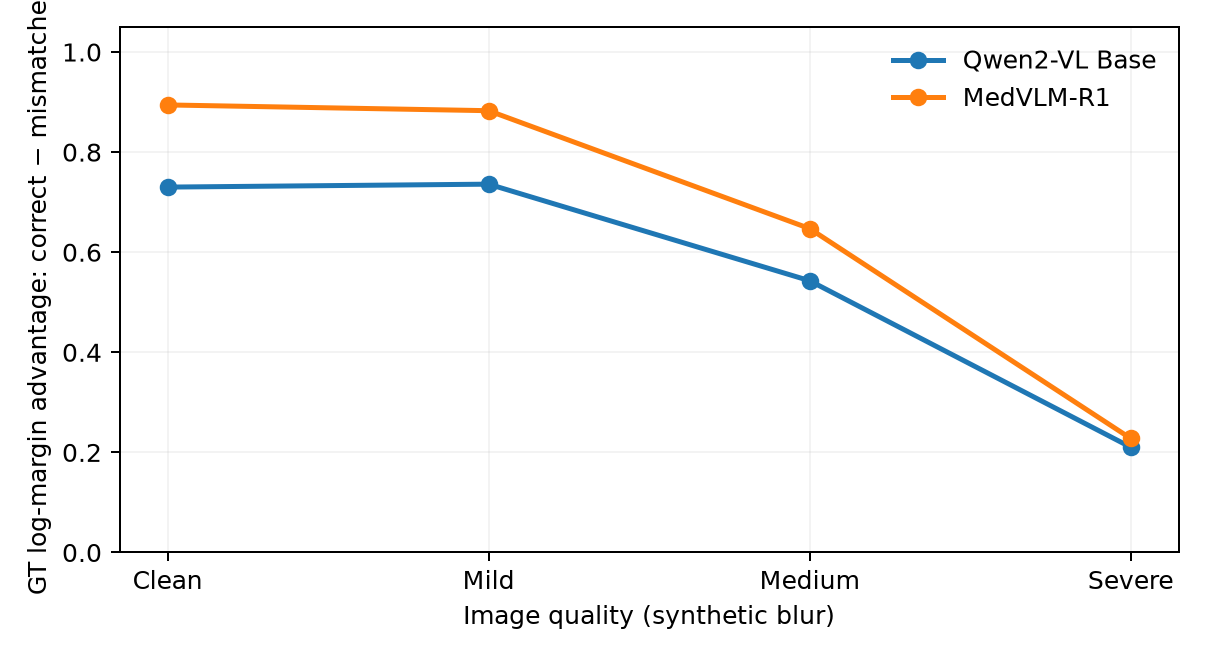
\includegraphics[keepaspectratio,alt={Correct-image
benefit across image-quality levels}]{figures/quality_content_gap.png}}
\caption{Correct-image benefit across image-quality levels}
\end{figure}

Correct-image advantage stayed similar under mild blur but decreased
substantially under stronger degradation, as candidate-answer entropy
increased. \textbf{The degradation weakens the predictive support
supplied by the correct image in both checkpoints.} The precise margin
definition, modality breakdown, and entropy measurements are in
\textbf{\hyperref[image-degradation-and-quality-by-relevance-design]{Appendix
2.1}} and \textbf{\hyperref[behavioral-quality-sensitivity]{Appendix
2.2}}.

\subsection{2.2. Visual--Text Evidence
Competition}\label{visualtext-evidence-competition}

We then asked whether weaker or mismatched visual evidence makes a model
more susceptible to \textbf{external textual advice}. We selected
\textbf{559 four-choice questions correctly answered with Clean images
by both checkpoints using the same candidate-scoring protocol}. For
every question, we separately suggested A, B, C, or D, with an adaptive
confidence computed from \textbf{each model's own Clean prediction
probability}. The numeric confidence was fixed for that model/question
across all visual conditions.

\textbf{Hint following rate} is the fraction of the three suggestions
\emph{different from the current no-hint predicted option} that cause
the model to switch to the suggested option:

{\def\LTcaptype{none} % do not increment counter
\begin{longtable}[]{@{}lrr@{}}
\toprule\noalign{}
Visual input & Qwen2-VL Base & MedVLM-R1 \\
\midrule\noalign{}
\endhead
\bottomrule\noalign{}
\endlastfoot
Clean & \textbf{66.1\%} & \textbf{40.5\%} \\
Severe Blur & 82.3\% & 66.3\% \\
Mismatch & 70.5\% & 48.7\% \\
No-image & 89.5\% & 81.8\% \\
\end{longtable}
}

Both models followed textual suggestions more often when the image was
severely blurred or removed. R1 followed advice less often under every
visual condition, while showing a larger \textbf{Clean-to-Severe
increase} (+25.82 percentage points {[}pp{]} versus +16.28 pp for Base).
Random Mismatch produced a smaller change. \textbf{The experiment
measures how strongly external text competes with image-conditioned
decisions.} Each checkpoint received confidence statements derived from
its own Clean predictions; the paired quality changes therefore provide
the clearest comparison of how susceptibility responds to image
degradation. Detailed controls and statistics appear in
\textbf{\hyperref[visualtext-evidence-competition-559-item-protocol]{Appendix
2.3--2.5}}.

\subsection{2.3. Decision-Token Intervention: Modulating Visual
Evidence}\label{decision-token-intervention-modulating-visual-evidence}

We further tested whether a quality-associated internal change can
affect the contribution of the current image \textbf{without changing
its pixels}. Using \textbf{450 separate questions} to estimate the mean
Severe-Blur-minus-Clean activation direction, we added this direction at
\textbf{decoder layer 27, at the final prompt/decision-token residual
state}, on \textbf{90 held-out questions per checkpoint}. The model
weights and the actual input image remained unchanged.

{\def\LTcaptype{none} % do not increment counter
\begin{longtable}[]{@{}
  >{\raggedright\arraybackslash}p{(\linewidth - 4\tabcolsep) * \real{0.2727}}
  >{\raggedleft\arraybackslash}p{(\linewidth - 4\tabcolsep) * \real{0.3636}}
  >{\raggedleft\arraybackslash}p{(\linewidth - 4\tabcolsep) * \real{0.3636}}@{}}
\toprule\noalign{}
\begin{minipage}[b]{\linewidth}\raggedright
L27 quality-direction intervention
\end{minipage} & \begin{minipage}[b]{\linewidth}\raggedleft
Qwen Base
\end{minipage} & \begin{minipage}[b]{\linewidth}\raggedleft
MedVLM-R1
\end{minipage} \\
\midrule\noalign{}
\endhead
\bottomrule\noalign{}
\endlastfoot
Change in correct-image content advantage (Clean − Mismatch GT log
margin) & \textbf{−0.131} & \textbf{−0.157} \\
Change in Clean GT log margin & −0.128 & −0.315 \\
Change in Clean answer entropy & +0.071 & +0.092 \\
\end{longtable}
}

The learned direction reduced the benefit of the correctly paired image
more than an equal-norm random direction, with a stronger response at
higher intervention doses. It also increased answer entropy in
\textbf{No-image} inputs (+0.058 for Base; +0.095 for R1).
\textbf{Decision-token representations modulate visual-content support
and broader answer uncertainty at the same time.} The full-state
replacement, held-out controls, and dose-response results are retained
in
\textbf{\hyperref[representation-evidence-quality-versus-content]{Appendix
2.6--2.9}}.

\subsection{2.4. Main Findings}\label{main-findings}

\textbf{(1) Image quality matters:} Both models lose correct-image
predictive advantage as blur becomes more severe. \textbf{(2) RL
strengthens image-conditioned decision stability while leaving
quality-aware reliance underdeveloped:} R1 follows competing textual
advice less often than Base under Clean, Severe Blur, and Mismatch. Its
stronger commitment persists with degraded or mismatched images, while
loss of visual evidence triggers substantial shifts, especially on MRI.
\textbf{(3) Medical RL improves task accuracy more than evidence
calibration:} R1 gains substantially even with No-image input, and the
extra benefit of supplying the correct image remains almost unchanged.
\textbf{Together, the results suggest that medical RL reinforces
image-conditioned decisions and task-specific priors more effectively
than reliable control over when and how much the image is trusted.}

\textbf{This leads to Part 3:} The next question is which capabilities
drive the large medical-VQA accuracy gains while quality-aware visual
reliance remains weak. We investigate image-free improvements, their
concentration in the MRI training modality, and whether the image-free
advantage persists even on questions both checkpoints already solve
correctly with Clean images.

\section{3. What Did RL Actually
Improve?}\label{what-did-rl-actually-improve}

\subsection{3.1. Substantial Gains Persist without
Images}\label{substantial-gains-persist-without-images}

The matched \textbf{825-question, four-choice} comparison shows that
MedVLM-R1 improves with the original image and achieves a gain of
similar magnitude with \textbf{No-image} input. Scores are averaged over
three fixed option orders for each question.

{\def\LTcaptype{none} % do not increment counter
\begin{longtable}[]{@{}lrrr@{}}
\toprule\noalign{}
Input condition & Qwen2-VL Base & MedVLM-R1 & RL − Base \\
\midrule\noalign{}
\endhead
\bottomrule\noalign{}
\endlastfoot
Clean image & 68.89\% & \textbf{80.97\%} & \textbf{+12.08 pp} \\
No-image & 44.12\% & \textbf{57.94\%} & \textbf{+13.82 pp} \\
Clean − No-image benefit & +24.77 pp & +23.03 pp & \textbf{−1.74 pp} \\
\end{longtable}
}

\textbf{The RL accuracy gain is reproduced at the same scale without any
image:} +13.82 pp in No-image versus +12.08 pp in Clean. The incremental
accuracy benefit of adding the current image changes by only −1.74 pp
(95\% paired CI {[}−3.80, +0.32{]}). The central improvement is a much
stronger ability to recover benchmark answers from \textbf{non-visual
signals}---medical knowledge, question wording, option plausibility, and
dataset-specific answer patterns. An answer-accuracy reward can
reinforce precisely these predictive patterns without requiring better
visual grounding. Detailed paired statistics are in
\textbf{\hyperref[matched-scoring-clean-versus-no-image]{Appendix 3.1}}.

\subsection{3.2. Gains Are Concentrated in the MRI Training
Modality}\label{gains-are-concentrated-in-the-mri-training-modality}

The original MedVLM-R1 GRPO training uses MRI examples. The matched
evaluation shows that its improvement is strongly concentrated in MRI,
both with and without images:

{\def\LTcaptype{none} % do not increment counter
\begin{longtable}[]{@{}lrr@{}}
\toprule\noalign{}
Modality & RL − Base, Clean & RL − Base, No-image \\
\midrule\noalign{}
\endhead
\bottomrule\noalign{}
\endlastfoot
\textbf{MRI (n=300)} & \textbf{+29.11 pp} & \textbf{+32.11 pp} \\
CT (n=237) & +4.36 pp & +5.49 pp \\
X-ray (n=288) & +0.69 pp & +1.62 pp \\
\end{longtable}
}

\textbf{MRI No-image accuracy reaches 75.67\% after RL, compared with
43.56\% for Base}, even though the diagnostic image is absent. The
No-image gain on MRI (+32.11 pp) is greater than the Clean gain (+29.11
pp), whereas the corresponding gains on CT and X-ray are much smaller.
This marked concentration in the \textbf{MRI training modality} points
to \textbf{reward-driven strengthening of MRI-specific medical and
benchmark question--answer regularities} as the dominant observed
post-training effect. The complete breakdown is in
\textbf{\hyperref[where-are-the-gains-concentrated-mri-versus-ct-and-x-ray]{Appendix
3.2}}.

\subsection{3.3. The No-Image Advantage Persists on Questions Both
Models Already
Solve}\label{the-no-image-advantage-persists-on-questions-both-models-already-solve}

We examined \textbf{559 four-choice questions that both models already
answered correctly with Clean images}, using the same O0
candidate-scoring protocol. We then removed the images and compared the
two checkpoints on these identical questions.

{\def\LTcaptype{none} % do not increment counter
\begin{longtable}[]{@{}
  >{\raggedright\arraybackslash}p{(\linewidth - 6\tabcolsep) * \real{0.2000}}
  >{\raggedleft\arraybackslash}p{(\linewidth - 6\tabcolsep) * \real{0.2667}}
  >{\raggedleft\arraybackslash}p{(\linewidth - 6\tabcolsep) * \real{0.2667}}
  >{\raggedleft\arraybackslash}p{(\linewidth - 6\tabcolsep) * \real{0.2667}}@{}}
\toprule\noalign{}
\begin{minipage}[b]{\linewidth}\raggedright
Clean-correct subset / No-image evaluation
\end{minipage} & \begin{minipage}[b]{\linewidth}\raggedleft
Qwen2-VL Base
\end{minipage} & \begin{minipage}[b]{\linewidth}\raggedleft
MedVLM-R1
\end{minipage} & \begin{minipage}[b]{\linewidth}\raggedleft
RL − Base
\end{minipage} \\
\midrule\noalign{}
\endhead
\bottomrule\noalign{}
\endlastfoot
\textbf{All 559 questions} & 51.52\% (288/559) & \textbf{62.25\%
(348/559)} & \textbf{+10.73 pp} \\
\textbf{MRI 207 questions} & 45.89\% (95/207) & \textbf{71.50\%
(148/207)} & \textbf{+25.60 pp} \\
\end{longtable}
}

The overall No-image advantage is \textbf{+10.73 pp} (95\% paired CI
{[}+7.87, +13.60{]}); \textbf{66} questions are answered correctly only
by R1 versus \textbf{6} only by Base. Importantly, \textbf{R1 retains
this advantage on questions Base could already answer with the original
image}. Combined with the particularly large MRI effect and the
final-answer accuracy reward, these results strengthen the case for
\textbf{reward-amplified learning of medical and dataset-specific
question--answer patterns} as a main source of the improved answer
recovery. The complete paired results and the older 506-item diagnostic
appear in
\textbf{\hyperref[matched-559-item-joint-clean-correct-subset]{Appendix
3.3--3.4}}.

\subsection{3.4. Interpretation: What the Reward
Encourages}\label{interpretation-what-the-reward-encourages}

MedVLM-R1's GRPO objective rewards \textbf{correct final answers and the
required output format}. It provides a strong incentive to learn medical
and dataset-specific patterns predictive of the answer, with no explicit
reward for matching the answer to reliable evidence in the current
image. The experiments reveal the expected consequence of that
incentive: \textbf{large accuracy gains survive image removal, are
concentrated in the MRI training modality, and persist even on questions
both models already solve with Clean images}. This strongly points to
\textbf{reward-driven fitting of non-visual medical and
benchmark-specific answer patterns} as a major contributor to the
observed gains. In short, \textbf{medical RL improves benchmark answer
selection while leaving calibration of visual-evidence trust as an unmet
training objective}. The reward design and a direct image-free RL
control are covered in
\textbf{\hyperref[why-the-medvlm-r1-reward-motivates-a-non-visual-prior-hypothesis]{Appendix
3.5--3.6}}.

\section{4. Does Medical RL Generalize Beyond the Training
Benchmark?}\label{does-medical-rl-generalize-beyond-the-training-benchmark}

\subsection{4.1. The MRI Gains Disappear on External Medical
VQA}\label{the-mri-gains-disappear-on-external-medical-vqa}

We evaluated the same Qwen2-VL Base and MedVLM-R1 checkpoints on
\textbf{SLAKE} (355 English Yes/No test questions) and \textbf{PMC-VQA}
(a frozen 1,000-question, four-choice test sample), keeping question
sets, visual interventions, and candidate scoring matched within each
dataset. We compare RL-minus-Base accuracy under the original image
(\textbf{Clean}) and with the image removed (\textbf{No-image}):

{\def\LTcaptype{none} % do not increment counter
\begin{longtable}[]{@{}lrr@{}}
\toprule\noalign{}
Evaluation set & RL − Base, Clean & RL − Base, No-image \\
\midrule\noalign{}
\endhead
\bottomrule\noalign{}
\endlastfoot
Original MRI benchmark (300) & \textbf{+29.11 pp} & \textbf{+32.11
pp} \\
\textbf{SLAKE (355)} & \textbf{−5.77 pp} & \textbf{−2.68 pp} \\
\textbf{PMC-VQA (1,000)} & \textbf{+0.33 pp} & \textbf{−0.37 pp} \\
\end{longtable}
}

The large MRI improvement \textbf{disappears on external benchmarks}: R1
performs \textbf{worse than Base on SLAKE} (Clean 62.25\% versus
68.03\%) and is approximately tied on PMC-VQA (45.43\% versus 45.10\%).
The strong MRI No-image advantage also disappears on both external
datasets. These results reinforce the Part 3 finding that
\textbf{medical RL rewards training-task-specific, non-visual answer
patterns more effectively than generalizable medical visual reasoning}.
Full accuracies, paired intervals, and evaluation protocols appear in
\textbf{\hyperref[external-datasets-and-matched-evaluation]{Appendix
4.1--4.2}}.

\subsection{4.2. The Image-Free Advantage Is Specific to the Original
Benchmark}\label{the-image-free-advantage-is-specific-to-the-original-benchmark}

We repeated the Part 3.3 analysis: restrict each dataset to questions
\textbf{both checkpoints answer correctly with Clean}, then measure
whether those correct answers survive image removal.

{\def\LTcaptype{none} % do not increment counter
\begin{longtable}[]{@{}
  >{\raggedright\arraybackslash}p{(\linewidth - 6\tabcolsep) * \real{0.2000}}
  >{\raggedleft\arraybackslash}p{(\linewidth - 6\tabcolsep) * \real{0.2667}}
  >{\raggedleft\arraybackslash}p{(\linewidth - 6\tabcolsep) * \real{0.2667}}
  >{\raggedleft\arraybackslash}p{(\linewidth - 6\tabcolsep) * \real{0.2667}}@{}}
\toprule\noalign{}
\begin{minipage}[b]{\linewidth}\raggedright
Jointly Clean-correct set
\end{minipage} & \begin{minipage}[b]{\linewidth}\raggedleft
Base No-image
\end{minipage} & \begin{minipage}[b]{\linewidth}\raggedleft
MedVLM-R1 No-image
\end{minipage} & \begin{minipage}[b]{\linewidth}\raggedleft
RL − Base
\end{minipage} \\
\midrule\noalign{}
\endhead
\bottomrule\noalign{}
\endlastfoot
Original MRI (207 questions) & 45.89\% & \textbf{71.50\%} &
\textbf{+25.60 pp} \\
SLAKE (209 questions) & 43.54\% & 42.58\% & −0.96 pp \\
PMC-VQA (448 questions) & 56.25\% & 55.58\% & −0.67 pp \\
\end{longtable}
}

\textbf{The strong image-free advantage exists on the original MRI task
but vanishes in both external jointly solvable subsets.} This isolates
the main generalization pattern: the RL checkpoint becomes substantially
better at selecting correct answers from the original task's text and
option cues, while its enhanced answer recovery fails to carry over to
other medical question distributions. See
\textbf{\hyperref[jointly-clean-correct-questions-on-external-data]{Appendix
4.3}}.

\subsection{4.3. Correct-Image Benefits Remain Similar after
RL}\label{correct-image-benefits-remain-similar-after-rl}

A shuffled-image control supplies a real medical image from a different
question while keeping an image in the model input. The \textbf{Clean −
Shuffled} accuracy gap measures how much the correct image--question
pairing helps answer selection:

{\def\LTcaptype{none} % do not increment counter
\begin{longtable}[]{@{}
  >{\raggedright\arraybackslash}p{(\linewidth - 4\tabcolsep) * \real{0.2727}}
  >{\raggedleft\arraybackslash}p{(\linewidth - 4\tabcolsep) * \real{0.3636}}
  >{\raggedleft\arraybackslash}p{(\linewidth - 4\tabcolsep) * \real{0.3636}}@{}}
\toprule\noalign{}
\begin{minipage}[b]{\linewidth}\raggedright
External dataset
\end{minipage} & \begin{minipage}[b]{\linewidth}\raggedleft
Base: Clean − Shuffled
\end{minipage} & \begin{minipage}[b]{\linewidth}\raggedleft
MedVLM-R1: Clean − Shuffled
\end{minipage} \\
\midrule\noalign{}
\endhead
\bottomrule\noalign{}
\endlastfoot
SLAKE & +15.21 pp & +13.10 pp \\
PMC-VQA & +15.77 pp & +16.03 pp \\
\end{longtable}
}

Both models benefit from correct visual content. \textbf{R1 produces no
consistent gain in that benefit after medical RL.} We also tested
\textbf{47 SLAKE pairs with identical question text and modality but
opposite dataset-annotated Yes/No answers}. The probability moved in the
label-consistent direction for \textbf{40/47 (85.11\%)} pairs under Base
and \textbf{38/47 (80.85\%)} under R1. This more tightly controlled
image-content comparison likewise favors \textbf{task-specific reward
learning over a general improvement in visual evidence use}. The paired
construction and VQA-RAD supplementary results are in
\textbf{\hyperref[image-content-relevance-and-opposite-label-pairs]{Appendix
4.4--4.5}}.

\section{5. Discussion and Research
Implications}\label{discussion-and-research-implications}

\subsection{5.1. Visual Evidence Is Used, but Reliance Is Poorly
Regulated}\label{visual-evidence-is-used-but-reliance-is-poorly-regulated}

Clean-to-Mismatch performance changes, quality degradation, text-advice
competition, and decision-token interventions all reveal
\textbf{behavioral and internal sensitivity to visual content}. The
remaining challenge is \textbf{evidence-dependent regulation}: the model
needs to reduce confidence in unreliable or irrelevant visual evidence
and prioritize the relevant evidence when it is diagnostic. R1's lower
susceptibility to competing text under degraded or mismatched images
suggests that medical RL may strengthen visual commitment
\textbf{without a corresponding improvement in reliability-aware
reliance}.

\subsection{5.2. Accuracy Rewards Reinforce Task-Specific Answer
Patterns}\label{accuracy-rewards-reinforce-task-specific-answer-patterns}

The central pattern now spans three tests: \textbf{(i)} No-image gains
on the original MRI benchmark rival Clean gains; \textbf{(ii)} those
gains remain on MRI questions both models already solve with Clean
images; and \textbf{(iii)} the gains disappear on SLAKE and PMC-VQA.
Together they point to \textbf{reward-amplified use of MRI-specific
medical, linguistic, and benchmark statistical regularities} as a major
source of post-training improvement. The reward improves answer
selection on the training-aligned task while leaving generalizable
visual-evidence calibration underdeveloped.

\subsection{5.3. The Evaluation Target Should Shift from Accuracy
Alone}\label{the-evaluation-target-should-shift-from-accuracy-alone}

Medical VQA accuracy should be accompanied by tests of
\textbf{correct-image contribution, visual degradation response,
image--question mismatch, and evidence conflicts}. These measurements
separate successful answer prediction from successful use of the current
medical image. They also identify a natural training target: reward
answers that follow reliable, task-relevant visual evidence, and
encourage appropriate uncertainty when that evidence becomes weak.

\section{6. Next Steps}\label{next-steps}

\textbf{Priority 1 --- Matched image-conditioned versus image-free RL.}
Starting from the same Base checkpoint and MRI questions, train two
policies with matched reward and optimization budget, one with images
and one without. Compare Clean, No-image, shuffled-image, and external
benchmark performance. This directly measures how much of the observed
gain the answer-accuracy reward can reproduce from non-visual signals
alone.

\textbf{Priority 2 --- Reliability-aware visual-evidence reward.} Build
a controlled training/evaluation set with image-quality gradients,
question--image consistency checks, and dataset-annotated
opposite-answer image pairs. Reward correct answers together with
\textbf{appropriate sensitivity to reliable visual evidence}; evaluate
answer accuracy, image-content advantage, and evidence-sensitive
confidence.

\textbf{Priority 3 --- Decision-token mechanism tests.} Extend the
layer-27 quality-direction intervention to larger independent evaluation
sets. Use dose-controlled steering, matched random directions, no-image
controls, and localized activation replacements to separate
visual-quality information from generic answer uncertainty and identify
more selective visual-evidence representations.

\textbf{Discussion focus.} Which next experiment best distinguishes
reward-amplified benchmark priors from improved image grounding, and
which visual-evidence reliability target is most useful for medical
applications?

\begin{center}\rule{0.5\linewidth}{0.5pt}\end{center}

\section{Appendix}\label{appendix}

\subsection{Appendix 0. Dataset, Image Interventions, and Evaluation
Protocol}\label{appendix-0.-dataset-image-interventions-and-evaluation-protocol}

\subsubsection{0.1. Models and evaluation
datasets}\label{models-and-evaluation-datasets}

We evaluate two released checkpoints from the same medical-VQA model
line:

\begin{itemize}
\tightlist
\item
  \textbf{Qwen2-VL-2B-Instruct (Base):} the general-purpose
  vision-language model before the medical-VQA RL post-training studied
  here.
\item
  \textbf{MedVLM-R1 (RL):} the medical-reasoning checkpoint trained with
  reinforcement learning, evaluated on the same questions and
  interventions as Base.
\end{itemize}

The main benchmark comes from the
\href{https://github.com/JZPeterPan/MedVLM-R1}{MedVLM-R1 official
evaluation set}. Its benchmark file is
\texttt{MRI\_CT\_XRAY\_300each\_dataset.json}. The images are provided
by the
\href{https://huggingface.co/datasets/FreedomIntelligence/Medical_Multimodal_Evaluation_Data}{Medical
Multimodal Evaluation Data} collection. Each of the \textbf{900
questions has its own paired image}, together with a question, answer
choices, and a reference answer.

The original benchmark contains both four-choice and two-choice
questions:

{\def\LTcaptype{none} % do not increment counter
\begin{longtable}[]{@{}lrrr@{}}
\toprule\noalign{}
Imaging modality & Four choices & Two choices & Total \\
\midrule\noalign{}
\endhead
\bottomrule\noalign{}
\endlastfoot
MRI & 300 & 0 & 300 \\
CT & 237 & 63 & 300 \\
X-ray & 288 & 12 & 300 \\
\textbf{Total} & \textbf{825} & \textbf{75} & \textbf{900} \\
\end{longtable}
}

We use the two evaluation sets for different purposes:

\begin{itemize}
\tightlist
\item
  \textbf{Official 900:} all MRI, CT, and X-ray questions, retaining
  each question's original number of options. This is the main
  population for image-quality and correct-image-versus-mismatched-image
  experiments.
\item
  \textbf{Four-choice 825:} the 825 items originally containing four
  answer options. This provides a uniform four-choice format for the
  principal Base/RL comparisons, including the full 300-question MRI
  block. For this subset, uniform random choice corresponds to
  \textbf{25\% accuracy}.
\end{itemize}

The 825-item subset is obtained by selecting the original four-choice
questions; the 75 two-choice questions remain in the 900-item quality
evaluation. Questions, option wording, and reference answers are
preserved. For additional transfer experiments, we use the English
Yes/No portion of \textbf{SLAKE} (355 test and 358 validation
questions), a fixed \textbf{1,000-question four-choice PMC-VQA} sample,
and \textbf{251 closed Yes/No VQA-RAD} questions. Their
benchmark-specific preparation is documented in the
\href{https://github.com/bbuller591-sketch/medical-vlm-visual-reliance/blob/main/docs/REPRODUCE_FROM_SCRATCH.md}{reproduction
guide}.

\subsubsection{0.2. Visual-input
interventions}\label{visual-input-interventions}

All interventions retain the original question, answer candidates, and
reference answer. We change the visual input to isolate different
aspects of image reliance.

{\def\LTcaptype{none} % do not increment counter
\begin{longtable}[]{@{}
  >{\raggedright\arraybackslash}p{(\linewidth - 4\tabcolsep) * \real{0.3333}}
  >{\raggedright\arraybackslash}p{(\linewidth - 4\tabcolsep) * \real{0.3333}}
  >{\raggedright\arraybackslash}p{(\linewidth - 4\tabcolsep) * \real{0.3333}}@{}}
\toprule\noalign{}
\begin{minipage}[b]{\linewidth}\raggedright
Condition
\end{minipage} & \begin{minipage}[b]{\linewidth}\raggedright
What the model receives
\end{minipage} & \begin{minipage}[b]{\linewidth}\raggedright
What the comparison measures
\end{minipage} \\
\midrule\noalign{}
\endhead
\bottomrule\noalign{}
\endlastfoot
\textbf{Clean} & The image originally paired with the question &
Performance with the correct visual evidence \\
\textbf{No-image} & The question and answer choices, with the image
omitted & Answering capability from non-visual input \\
\textbf{Blank} & A blank image with the question and choices & Effect of
an image channel carrying minimal visual content \\
\textbf{Mismatch} & A different real medical image paired with the same
question & Dependence on the correct image--question pairing \\
\textbf{Blur} & The original image with mild, medium, or severe Gaussian
blur & How image degradation changes performance and visual benefit \\
\textbf{Semantic conflict} & A replacement image selected using
conflicting dataset answer labels & Sensitivity to a more targeted
change in visual evidence \\
\end{longtable}
}

\textbf{Illustrative four-choice example (for explanation, separate from
the benchmark):}

\begin{quote}
\textbf{Question:} What finding is shown on this chest X-ray?

\begin{itemize}
\tightlist
\item
  A. Pneumothorax
\item
  B. Pleural effusion
\item
  C. Lung consolidation
\item
  D. No evident abnormality
\end{itemize}

\textbf{Reference answer:} B. Pleural effusion
\end{quote}

For \textbf{Clean}, the model sees the corresponding chest X-ray showing
a pleural effusion. For \textbf{No-image}, it receives the same question
and four options with the image removed. For \textbf{Mismatch}, the
image is replaced with another chest X-ray---for example, one showing a
pneumothorax---while the original question, options, and reference
answer stay fixed. For \textbf{Blur}, the original X-ray is
progressively blurred. A \textbf{Blank} input supplies an uninformative
image instead. The example illustrates how answer predictions can change
with the visual evidence even though the text remains identical.

In the full quality experiment, Mismatch uses \textbf{three fixed
same-modality real-image donors per question}. The correctly paired
image and donor images receive the \textbf{same blur level} when
evaluated at a particular quality setting. Semantic-conflict donors form
a separate, label-guided analysis. The synthetic Gaussian blur ladder is
fixed at mild, medium, and severe strengths, with a radius equal to
\textbf{0.005, 0.015, or 0.030 times the shorter image dimension},
respectively.

\subsubsection{0.3. Common answer-scoring and model-input
protocol}\label{common-answer-scoring-and-model-input-protocol}

For matched comparisons, both models receive the same question,
candidate answer texts, and image condition. Questions are formatted
with labeled options (for example, \texttt{A)\ ...}, \texttt{B)\ ...},
\texttt{C)\ ...}, \texttt{D)\ ...}). The model is prompted to answer
with a \textbf{single option letter}.

To measure candidate-answer probabilities, we extract the model's scores
for the applicable option letters and normalize them \textbf{within that
question's candidate set}. Predictions are then translated back into
their original option identities before computing accuracy,
correct-answer margins, and answer entropy.

We also control for answer-position effects:

\begin{itemize}
\tightlist
\item
  \textbf{Four-choice questions:} the original order, a deterministic
  cyclic rotation, and a seeded random permutation (three orderings).
\item
  \textbf{Two-choice questions:} the original and swapped arrangements
  are the two distinct possibilities. The full 900-question quality run
  uses three fixed order IDs; on two-choice items, the third ID repeats
  one of these arrangements.
\end{itemize}

The direct Base/RL candidate-scoring comparisons use matched
image-processor settings (\textbf{minimum 3,136 pixels; maximum 401,408
pixels}) so both checkpoints receive comparable visual-input budgets.
Original model-specific generation analyses are tracked separately and
identified with their own scoring protocol when presented in later
sections.

The same item IDs, answers, image-donor assignments, and option-order
controls are held fixed across model comparisons. The next sections
analyze how predictions change when the visual input changes, how these
effects depend on image quality, and how they differ between Base and
the RL checkpoint.

\subsection{Appendix 1. Behavioral Evidence for Reliance on the Current
Image}\label{appendix-1.-behavioral-evidence-for-reliance-on-the-current-image}

\subsubsection{1.1. Full-set visual-input interventions (825 four-choice
questions)}\label{full-set-visual-input-interventions-825-four-choice-questions}

The original experiment evaluated each checkpoint on the \textbf{same
825 original four-choice questions} under Clean, No-image, and a fixed
real-image Mismatch condition (\texttt{pm\_clean\_k1}). Mismatch keeps
the question, answer candidates, and reference label unchanged and
replaces the original image with another medical image.

{\def\LTcaptype{none} % do not increment counter
\begin{longtable}[]{@{}
  >{\raggedright\arraybackslash}p{(\linewidth - 6\tabcolsep) * \real{0.2000}}
  >{\raggedleft\arraybackslash}p{(\linewidth - 6\tabcolsep) * \real{0.2667}}
  >{\raggedleft\arraybackslash}p{(\linewidth - 6\tabcolsep) * \real{0.2667}}
  >{\raggedleft\arraybackslash}p{(\linewidth - 6\tabcolsep) * \real{0.2667}}@{}}
\toprule\noalign{}
\begin{minipage}[b]{\linewidth}\raggedright
Checkpoint and original scoring protocol
\end{minipage} & \begin{minipage}[b]{\linewidth}\raggedleft
Clean accuracy
\end{minipage} & \begin{minipage}[b]{\linewidth}\raggedleft
No-image accuracy
\end{minipage} & \begin{minipage}[b]{\linewidth}\raggedleft
Mismatch accuracy
\end{minipage} \\
\midrule\noalign{}
\endhead
\bottomrule\noalign{}
\endlastfoot
Qwen2-VL Base · candidate scoring & \textbf{64.73\%} (825/825 valid) &
43.39\% (825/825) & 50.18\% (825/825) \\
MedVLM-R1 · native answer generation & \textbf{81.46\%} (820/825 valid)
& 55.69\% (817/825) & 69.58\% (812/825) \\
\end{longtable}
}

The fractions in parentheses report \textbf{valid outputs / 825
attempted questions}. The original MedVLM-R1 run used native answer
generation; the Qwen2-VL run used direct candidate scoring. The
following deltas are computed \textbf{within each checkpoint}, using the
corresponding arm-specific accuracies. Direct Base/RL post-training
comparisons use the matched-scoring measurements in \textbf{Part 3.1 and
Appendix 3.1}.

For each model, define two complementary accuracy contrasts:

\[\begin{aligned}
\Delta_{\mathrm{presence}} &= \mathrm{Acc}(\mathrm{Clean})-\mathrm{Acc}(\mathrm{NoImage}),\\
\Delta_{\mathrm{content}} &= \mathrm{Acc}(\mathrm{Clean})-\mathrm{Acc}(\mathrm{Mismatch}).
\end{aligned}\]

{\def\LTcaptype{none} % do not increment counter
\begin{longtable}[]{@{}
  >{\raggedright\arraybackslash}p{(\linewidth - 6\tabcolsep) * \real{0.2000}}
  >{\raggedleft\arraybackslash}p{(\linewidth - 6\tabcolsep) * \real{0.2667}}
  >{\raggedleft\arraybackslash}p{(\linewidth - 6\tabcolsep) * \real{0.2667}}
  >{\raggedleft\arraybackslash}p{(\linewidth - 6\tabcolsep) * \real{0.2667}}@{}}
\toprule\noalign{}
\begin{minipage}[b]{\linewidth}\raggedright
Checkpoint
\end{minipage} & \begin{minipage}[b]{\linewidth}\raggedleft
Clean − No-image
\end{minipage} & \begin{minipage}[b]{\linewidth}\raggedleft
Clean − Mismatch
\end{minipage} & \begin{minipage}[b]{\linewidth}\raggedleft
Mismatch − No-image
\end{minipage} \\
\midrule\noalign{}
\endhead
\bottomrule\noalign{}
\endlastfoot
Qwen2-VL Base & \textbf{+21.34 pp} & \textbf{+14.55 pp} & +6.79 pp \\
MedVLM-R1 & \textbf{+25.77 pp} & \textbf{+11.88 pp} & +13.89 pp \\
\end{longtable}
}

The first contrast measures the accuracy difference between
\textbf{Clean and No-image inputs}. The second isolates the benefit of
the \textbf{correct image--question pairing} relative to another real
medical image, while retaining visual input in both conditions. The
third comparison quantifies how the presence of a mismatched image
changes performance relative to a text-only question. All three are
behavioral differences in answer accuracy, measured on the fixed
four-choice benchmark.

\subsubsection{1.2. Retention of correct answers under visual
interventions (506
questions)}\label{retention-of-correct-answers-under-visual-interventions-506-questions}

To address what happens \textbf{when the model initially answers
correctly}, we selected the \textbf{506 questions on which both Base and
MedVLM-R1 answered correctly with the original Clean image}. This
selection was made using Clean outcomes from the original
checkpoint-specific experiments, before examining No-image or Mismatch
predictions. The 506-question subset contains \textbf{192 MRI, 137 CT,
and 177 X-ray questions}.

For each subsequent input condition, \textbf{retention} is the fraction
of valid predictions that remain correct against the original reference
answer. The table shows both the number of correct retained answers and
the valid denominator.

{\def\LTcaptype{none} % do not increment counter
\begin{longtable}[]{@{}
  >{\raggedright\arraybackslash}p{(\linewidth - 4\tabcolsep) * \real{0.2727}}
  >{\raggedleft\arraybackslash}p{(\linewidth - 4\tabcolsep) * \real{0.3636}}
  >{\raggedleft\arraybackslash}p{(\linewidth - 4\tabcolsep) * \real{0.3636}}@{}}
\toprule\noalign{}
\begin{minipage}[b]{\linewidth}\raggedright
Intervention
\end{minipage} & \begin{minipage}[b]{\linewidth}\raggedleft
Qwen2-VL Base: correct / valid (retention)
\end{minipage} & \begin{minipage}[b]{\linewidth}\raggedleft
MedVLM-R1: correct / valid (retention)
\end{minipage} \\
\midrule\noalign{}
\endhead
\bottomrule\noalign{}
\endlastfoot
Clean & 506/506 (\textbf{100\%}) & 506/506 (\textbf{100\%}) \\
No-image & 269/506 (\textbf{53.2\%}) & 301/499 (\textbf{60.3\%}) \\
White blank image & 274/506 (\textbf{54.2\%}) & 310/502
(\textbf{61.8\%}) \\
Mean-color blank image & 261/506 (\textbf{51.6\%}) & 313/503
(\textbf{62.2\%}) \\
Mismatch (real medical image) & 344/506 (\textbf{68.0\%}) & 390/499
(\textbf{78.2\%}) \\
Label-supported semantic conflict & 145/223 (\textbf{65.0\%}) & 175/223
(\textbf{78.5\%}) \\
\end{longtable}
}

The semantic-conflict comparison is evaluated on the \textbf{223
selected questions} for which a label-supported donor was available. An
additional pure-noise-image control in the original MedVLM-R1 run
retained \textbf{309/493 (62.7\%)} correct answers.

\begin{figure}
\centering
\pandocbounded{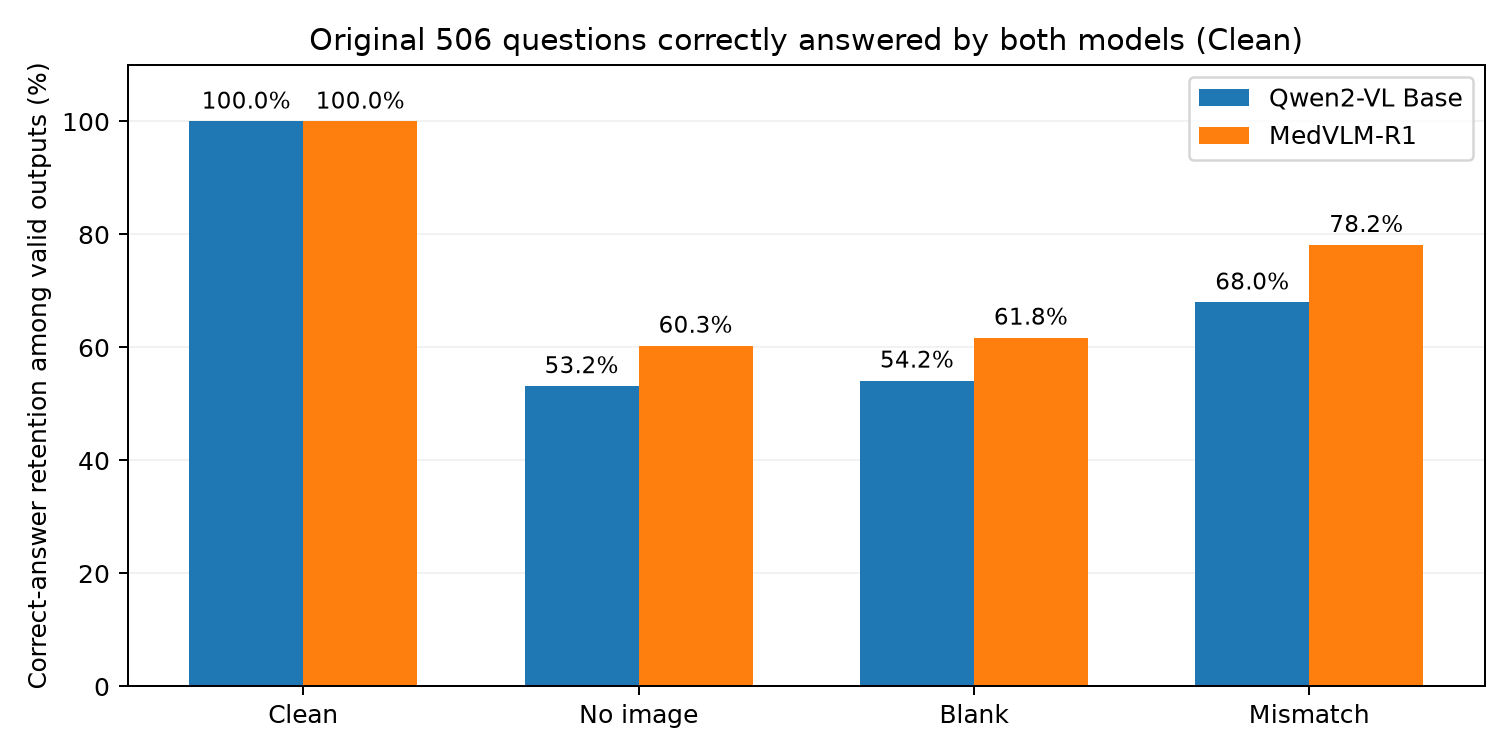
\includegraphics[keepaspectratio,alt={Clean-success
answer retention under image
interventions}]{figures/clean_correct_506_retention.png}}
\caption{Clean-success answer retention under image interventions}
\end{figure}

\emph{Each bar uses the valid denominator for that checkpoint and
condition; precise counts are provided above. The plotted conditions are
Clean, No-image, White blank, and Mismatch.}

On the \textbf{499 questions with valid No-image results from both
checkpoints}, MedVLM-R1 retained \textbf{301/499 (60.3\%)} correct
answers and Qwen2-VL Base retained \textbf{265/499 (53.1\%)}. Within
this paired set, 219 remained correct for both checkpoints, 82 only for
MedVLM-R1, 46 only for Base, and 152 for neither. This paired accounting
also informs the RL-focused analysis in \textbf{Appendix 3.4}.

These results show that many originally correct answers change when the
visual input is removed or replaced. In particular, a real but
mismatched medical image often preserves more correct answers than a
text-only or blank-image input, yet the correctly paired Clean image
produces the highest retention.

\subsubsection{1.3. Separating image presence from correct-image
content}\label{separating-image-presence-from-correct-image-content}

The image interventions answer related but distinct questions:

{\def\LTcaptype{none} % do not increment counter
\begin{longtable}[]{@{}
  >{\raggedright\arraybackslash}p{(\linewidth - 2\tabcolsep) * \real{0.5000}}
  >{\raggedright\arraybackslash}p{(\linewidth - 2\tabcolsep) * \real{0.5000}}@{}}
\toprule\noalign{}
\begin{minipage}[b]{\linewidth}\raggedright
Contrast
\end{minipage} & \begin{minipage}[b]{\linewidth}\raggedright
Question answered
\end{minipage} \\
\midrule\noalign{}
\endhead
\bottomrule\noalign{}
\endlastfoot
\textbf{Clean vs No-image} & How much does supplying the original image
change performance compared with answering from text alone? \\
\textbf{Clean vs Mismatch} & How much extra value comes from using the
image correctly paired with this question? \\
\textbf{Mismatch vs No-image} & How does an unrelated real medical image
change the model's prediction compared with having no visual input? \\
\textbf{Blank vs No-image} & How does an image input channel without
useful image content affect the prediction? \\
\end{longtable}
}

The Clean--Mismatch contrast is especially useful for studying
\textbf{current-image content} because both conditions provide real
images and differ in which image is paired with the fixed question. The
506-question analysis additionally conditions the experiment on
\textbf{initial Clean success}, directly tracing how correct answers
respond to visual interventions. Part 2 builds on this approach by
applying identical blur levels to both the correct and mismatched images
and measuring how their difference evolves with image quality.

\textbf{Data and figure provenance.} The original 825-item arm totals
and the original 506-item conditional counts are released as
\href{https://github.com/bbuller591-sketch/medical-vlm-visual-reliance/blob/main/results/official825_visual_interventions.csv}{\texttt{official825\_visual\_interventions.csv}}
and
\href{https://github.com/bbuller591-sketch/medical-vlm-visual-reliance/blob/main/results/clean_correct_506_interventions.csv}{\texttt{clean\_correct\_506\_interventions.csv}}.
The grouped chart is regenerated from the latter with
\href{https://github.com/bbuller591-sketch/medical-vlm-visual-reliance/blob/main/scripts/plot_clean_correct_506.py}{\texttt{plot\_clean\_correct\_506.py}}.

\subsection{Appendix 2. Image Quality, Visual--Text Competition, and
Decision-Token
Interventions}\label{appendix-2.-image-quality-visualtext-competition-and-decision-token-interventions}

\subsubsection{2.1. Image degradation and quality-by-relevance
design}\label{image-degradation-and-quality-by-relevance-design}

The main quality experiment uses all \textbf{900 official questions},
including the original two-choice and four-choice formats. Gaussian blur
is applied at matched levels to the correctly paired images and three
fixed, same-modality, incorrectly paired donor images. Questions,
choices, and reference labels stay unchanged. A correct image and its
mismatched donor are compared \textbf{at the same image-quality level}.

{\def\LTcaptype{none} % do not increment counter
\begin{longtable}[]{@{}
  >{\raggedright\arraybackslash}p{(\linewidth - 4\tabcolsep) * \real{0.2727}}
  >{\raggedleft\arraybackslash}p{(\linewidth - 4\tabcolsep) * \real{0.3636}}
  >{\raggedleft\arraybackslash}p{(\linewidth - 4\tabcolsep) * \real{0.3636}}@{}}
\toprule\noalign{}
\begin{minipage}[b]{\linewidth}\raggedright
Quality level
\end{minipage} & \begin{minipage}[b]{\linewidth}\raggedleft
Approximate Gaussian sigma
\end{minipage} & \begin{minipage}[b]{\linewidth}\raggedleft
Image-space SSIM vs original (mean over 900)
\end{minipage} \\
\midrule\noalign{}
\endhead
\bottomrule\noalign{}
\endlastfoot
Clean & 0 px & 1.000 \\
Mild blur & 2 px & 0.874 \\
Intermediate sensitivity check & 4 px & 0.769 \\
Medium blur & 6 px & 0.708 \\
Severe blur & 12 px & 0.617 \\
\end{longtable}
}

The intermediate 4-pixel condition was added as a sensitivity check
after the original four-level design. The original fixed blur parameters
scale with the image's shorter dimension, yielding these approximate
average pixel radii.

Let \(y^*\) denote the ground-truth answer among the original candidate
options. The signed GT log margin compares the correct answer with its
strongest competitor:

\[M_{\log}=\log p(y^*)-\max_{y\ne y^*}\log p(y).\]

The content advantage at quality level \(q\) compares the paired image's
margin against the mean over \(K=3\) mismatched donors:

\[U_{\mathrm{content}}(q)=M_{\log}(I_{\mathrm{correct}},q)-\frac{1}{K}\sum_{k=1}^{K}M_{\log}(I_{\mathrm{mismatch},k},q),\qquad K=3.\]

The first quantity measures correct-answer support; the second
specifically measures the value of the \textbf{correctly paired image
content}, relative to alternative real medical images under equal
degradation.

\subsubsection{2.2. Behavioral quality
sensitivity}\label{behavioral-quality-sensitivity}

The following table reports the mean \(U_{\mathrm{content}}\) across all
900 questions. Each cell averages three fixed donor comparisons with
matched image preprocessing and candidate-answer scoring.

{\def\LTcaptype{none} % do not increment counter
\begin{longtable}[]{@{}
  >{\raggedright\arraybackslash}p{(\linewidth - 10\tabcolsep) * \real{0.1304}}
  >{\raggedleft\arraybackslash}p{(\linewidth - 10\tabcolsep) * \real{0.1739}}
  >{\raggedleft\arraybackslash}p{(\linewidth - 10\tabcolsep) * \real{0.1739}}
  >{\raggedleft\arraybackslash}p{(\linewidth - 10\tabcolsep) * \real{0.1739}}
  >{\raggedleft\arraybackslash}p{(\linewidth - 10\tabcolsep) * \real{0.1739}}
  >{\raggedleft\arraybackslash}p{(\linewidth - 10\tabcolsep) * \real{0.1739}}@{}}
\toprule\noalign{}
\begin{minipage}[b]{\linewidth}\raggedright
Model
\end{minipage} & \begin{minipage}[b]{\linewidth}\raggedleft
Clean
\end{minipage} & \begin{minipage}[b]{\linewidth}\raggedleft
Mild (2 px)
\end{minipage} & \begin{minipage}[b]{\linewidth}\raggedleft
Extra (4 px)
\end{minipage} & \begin{minipage}[b]{\linewidth}\raggedleft
Medium (6 px)
\end{minipage} & \begin{minipage}[b]{\linewidth}\raggedleft
Severe (12 px)
\end{minipage} \\
\midrule\noalign{}
\endhead
\bottomrule\noalign{}
\endlastfoot
Qwen2-VL Base & 0.730 & 0.736 & 0.599 & 0.543 & 0.211 \\
MedVLM-R1 & 0.894 & 0.883 & 0.742 & 0.647 & 0.228 \\
\end{longtable}
}

A visible decrease is already present in the 4-pixel sensitivity
condition, while the mild-blur contrast stays close to Clean. Effects
vary by imaging modality:

{\def\LTcaptype{none} % do not increment counter
\begin{longtable}[]{@{}
  >{\raggedright\arraybackslash}p{(\linewidth - 4\tabcolsep) * \real{0.2727}}
  >{\raggedleft\arraybackslash}p{(\linewidth - 4\tabcolsep) * \real{0.3636}}
  >{\raggedleft\arraybackslash}p{(\linewidth - 4\tabcolsep) * \real{0.3636}}@{}}
\toprule\noalign{}
\begin{minipage}[b]{\linewidth}\raggedright
Model / modality
\end{minipage} & \begin{minipage}[b]{\linewidth}\raggedleft
Clean content advantage
\end{minipage} & \begin{minipage}[b]{\linewidth}\raggedleft
Severe-blur content advantage
\end{minipage} \\
\midrule\noalign{}
\endhead
\bottomrule\noalign{}
\endlastfoot
Base / MRI & 0.610 & 0.127 \\
Base / CT & 0.533 & 0.165 \\
Base / X-ray & 1.047 & 0.340 \\
MedVLM-R1 / MRI & 0.797 & 0.101 \\
MedVLM-R1 / CT & 0.656 & 0.179 \\
MedVLM-R1 / X-ray & 1.230 & 0.404 \\
\end{longtable}
}

In the earlier 825-question model-specific intervention run, mean GT log
margin decreased from \textbf{1.045 to 0.333} for Base and from
\textbf{4.102 to 2.184} for MedVLM-R1 between Clean and severe blur. In
the matched-scoring quality analysis, mean answer entropy increased from
\textbf{0.756 to 0.972} for Base and from \textbf{0.220 to 0.362} for
MedVLM-R1. These measurements connect decreasing correct-answer support
with increasing answer uncertainty.

For a complementary confidence/evidence diagnostic, define image-induced
entropy reduction and utility relative to No-image:

\[\Delta H=H(p_{\mathrm{NoImage}})-H(p_{\mathrm{Image}}),\qquad
U_{\mathrm{presence}}=M_{\log}(p_{\mathrm{Image}})-M_{\log}(p_{\mathrm{NoImage}}).\]

On \textbf{375 label-supported semantic-conflict cases} with
Clean-quality images, adding the image \textbf{reduced entropy while
also lowering GT margin} in \textbf{30.7\%} of Base cases and
\textbf{23.5\%} of MedVLM-R1 cases. Image-induced confidence and
answer-relevant visual utility therefore have measurably different
behavior.

\subsubsection{2.3. Visual--text evidence competition: 559-item
protocol}\label{visualtext-evidence-competition-559-item-protocol}

The advice experiment reuses the \textbf{825 original four-option
items}, with the \textbf{O0/original answer order} and identical
four-option candidate-probability scoring for Base and R1. An item is
included only if \textbf{both models predict the ground-truth option
correctly on Clean} using this scoring procedure, before inspecting any
advice-intervention outcome. This yields \textbf{559 common questions}:
207 MRI, 160 CT, and 192 X-ray. The earlier 506-item group in Part 1
used a native-generation/direct-scoring combination; the current
559-item group applies matched candidate scoring to both checkpoints. We
use the same questions and visual images for both checkpoints.

For each model \(m\) and question \(i\), let \(x_{i,m}\) be its
\textbf{highest four-option probability in percent under Clean, no
advice}; on this preselected set the highest option is the original
reference. Define the confidence in the advice statement as

\(c_{i,m}=25+0.5(x_{i,m}-25)\) (percent).

Average advice confidence is \textbf{49.69\% for Base} and
\textbf{56.07\% for R1}. The two checkpoints intentionally receive
\emph{their own} confidence values, as specified in the design. Each
confidence is frozen across every visual condition and every hinted
semantic option for that item and checkpoint. The prompt appends the
following sentence to the original question/answer choices, before the
unchanged single-letter response instruction:

\begin{quote}
I am \{confidence\}\% confident that option \{letter\} is correct, but I
may be wrong. Please make your own judgment based on the available
evidence.
\end{quote}

Four separate runs suggest A, B, C and D, regardless of whether the
suggestion is correct, plus one no-hint baseline. The frozen condition
set contains Clean, Severe Blur, random same-modality Mismatch, Blur
applied to that same Mismatch, and genuine No-image (no image tokens).
\textbf{Blur + Mismatch is retained in the data and appendix as a
supplementary factorial check but omitted from the compact Part 2.2
table.} All image degradation assets and mismatched donor assignments
were reused from the earlier frozen experiments; the new combined arm
was generated deterministically. Severe blur uses
\(\sigma=0.03\min(w,h)\) of the source image size. The text-advice
results were evaluated once in a balanced 30-item pilot and then on the
\textbf{entire 559-item eligible cohort}, using a fixed protocol and no
post-hoc item selection.

The resulting dataset has \textbf{559 × 5 visual conditions × 5 prompt
settings × 2 checkpoints = 27,950 scored predictions}, with no duplicate
or missing item/condition/hint combinations. Clean no-hint predictions
and probabilities were verified against the frozen source scores. Note
that this 559-item intervention uses one original option order, while
the 825-item matched RL accuracy comparison below averages three option
orders.

\subsubsection{2.4. Hint-following metrics and complete behavioral
results}\label{hint-following-metrics-and-complete-behavioral-results}

Let \(\widehat y_{i,m,v}^{(0)}\) denote the four-option \emph{no-hint}
predicted answer under visual condition \(v\), and
\(\widehat y_{i,m,v}^{(h)}\) the prediction after text suggests option
\(h\). The \textbf{primary hint-following rate} averages, per question,
over the three suggestions different from that question's no-hint
answer:

\(S_{i,m,v}=\frac{1}{3}\sum_{h\ne\widehat y_{i,m,v}^{(0)}}\mathbf{1}[\widehat y_{i,m,v}^{(h)}=h]\).

The one suggestion repeating the model's current prediction is excluded,
leaving three suggestions that can produce an identifiable answer
switch. The per-question fraction is averaged over the \textbf{same 559
questions}. Because the no-hint answer can change after image
degradation, the excluded option is determined \textbf{separately for
each visual condition}. A high follow rate indicates stronger
\textbf{susceptibility to the fixed textual suggestion}.

{\def\LTcaptype{none} % do not increment counter
\begin{longtable}[]{@{}
  >{\raggedright\arraybackslash}p{(\linewidth - 8\tabcolsep) * \real{0.1579}}
  >{\raggedleft\arraybackslash}p{(\linewidth - 8\tabcolsep) * \real{0.2105}}
  >{\raggedleft\arraybackslash}p{(\linewidth - 8\tabcolsep) * \real{0.2105}}
  >{\raggedleft\arraybackslash}p{(\linewidth - 8\tabcolsep) * \real{0.2105}}
  >{\raggedleft\arraybackslash}p{(\linewidth - 8\tabcolsep) * \real{0.2105}}@{}}
\toprule\noalign{}
\begin{minipage}[b]{\linewidth}\raggedright
Visual condition
\end{minipage} & \begin{minipage}[b]{\linewidth}\raggedleft
Base: follow
\end{minipage} & \begin{minipage}[b]{\linewidth}\raggedleft
R1: follow
\end{minipage} & \begin{minipage}[b]{\linewidth}\raggedleft
Base: hinted non-reference option probability lift
\end{minipage} & \begin{minipage}[b]{\linewidth}\raggedleft
R1: lift
\end{minipage} \\
\midrule\noalign{}
\endhead
\bottomrule\noalign{}
\endlastfoot
Clean & 66.07\% & 40.49\% & +37.68 pp & +30.83 pp \\
Severe Blur & 82.35\% & 66.31\% & +40.79 pp & +39.93 pp \\
Random same-modality Mismatch & 70.54\% & 48.66\% & +36.99 pp & +32.19
pp \\
\textbf{Blur + Mismatch (supplementary)} & 83.24\% & 68.10\% & +40.59 pp
& +40.06 pp \\
No-image & 89.51\% & 81.81\% & +43.52 pp & +46.00 pp \\
\end{longtable}
}

Probability lift is measured as the \emph{change in probability of the
suggested option compared with no hint}, averaged over the three options
different from the \textbf{original gold answer} (semantic indices are
held fixed). It is a complementary continuous metric. The original
reference answer belongs to the original image; the randomly mismatched
image supplies alternative medical content with its own unknown answer
to the fixed question.

For initially correct final answers we separately compute a
\textbf{correct-to-wrong rate}: among question/condition pairs whose
\textbf{no-hint prediction equals the original reference}, the fraction
of three suggestions of non-reference options after which the prediction
is incorrect. Therefore the denominator depends on the visual condition,
even though the same original 559 items are tracked:

{\def\LTcaptype{none} % do not increment counter
\begin{longtable}[]{@{}
  >{\raggedright\arraybackslash}p{(\linewidth - 8\tabcolsep) * \real{0.1579}}
  >{\raggedleft\arraybackslash}p{(\linewidth - 8\tabcolsep) * \real{0.2105}}
  >{\raggedleft\arraybackslash}p{(\linewidth - 8\tabcolsep) * \real{0.2105}}
  >{\raggedleft\arraybackslash}p{(\linewidth - 8\tabcolsep) * \real{0.2105}}
  >{\raggedleft\arraybackslash}p{(\linewidth - 8\tabcolsep) * \real{0.2105}}@{}}
\toprule\noalign{}
\begin{minipage}[b]{\linewidth}\raggedright
Visual condition
\end{minipage} & \begin{minipage}[b]{\linewidth}\raggedleft
Base no-hint originally correct
\end{minipage} & \begin{minipage}[b]{\linewidth}\raggedleft
Base correct→wrong
\end{minipage} & \begin{minipage}[b]{\linewidth}\raggedleft
R1 no-hint originally correct
\end{minipage} & \begin{minipage}[b]{\linewidth}\raggedleft
R1 correct→wrong
\end{minipage} \\
\midrule\noalign{}
\endhead
\bottomrule\noalign{}
\endlastfoot
Clean & 559/559 & 68.63\% & 559/559 & 42.93\% \\
Severe Blur & 398/559 & 79.65\% & 446/559 & 63.30\% \\
No-image & 288/559 & 85.30\% & 348/559 & 77.20\% \\
\end{longtable}
}

These are proportions of eligible \textbf{wrong-advice trials}, with the
denominator determined by the number of originally correct no-hint
predictions in each visual condition. For random Mismatch, answer
changes measure the effect of substituting different medical content.
\textbf{Answer stability}, the maximum share of any one selected option
among all four prompted runs, supplies an additional descriptive check:
Clean Base 49.6\% versus R1 68.6\%, dropping to No-image Base 32.6\%
versus R1 38.3\%.

\subsubsection{2.5. Paired quality effects, model comparison, and
modality
breakdown}\label{paired-quality-effects-model-comparison-and-modality-breakdown}

For a given question, model, and visual condition we subtract the
\textbf{same model's Clean} hint-following rate
\(S_{i,m,\mathrm{Clean}}\). This controls the baseline susceptibility of
each question/checkpoint; the \emph{difference of these changes} (R1
minus Base) compares checkpoint responses to the same visual
manipulation. Paired 95\% confidence intervals resample the same
question IDs (4,000 bootstrap draws in the advice analysis).

{\def\LTcaptype{none} % do not increment counter
\begin{longtable}[]{@{}
  >{\raggedright\arraybackslash}p{(\linewidth - 6\tabcolsep) * \real{0.2000}}
  >{\raggedleft\arraybackslash}p{(\linewidth - 6\tabcolsep) * \real{0.2667}}
  >{\raggedleft\arraybackslash}p{(\linewidth - 6\tabcolsep) * \real{0.2667}}
  >{\raggedleft\arraybackslash}p{(\linewidth - 6\tabcolsep) * \real{0.2667}}@{}}
\toprule\noalign{}
\begin{minipage}[b]{\linewidth}\raggedright
Condition − Clean
\end{minipage} & \begin{minipage}[b]{\linewidth}\raggedleft
Base change
\end{minipage} & \begin{minipage}[b]{\linewidth}\raggedleft
R1 change
\end{minipage} & \begin{minipage}[b]{\linewidth}\raggedleft
R1 − Base in change (95\% CI, pp)
\end{minipage} \\
\midrule\noalign{}
\endhead
\bottomrule\noalign{}
\endlastfoot
Severe Blur & +16.28 pp & +25.82 pp & \textbf{+9.54} {[}+6.98,
+12.10{]} \\
Random Mismatch & +4.47 pp & +8.17 pp & +3.70 {[}+1.19, +6.26{]} \\
Supplementary Blur + Mismatch & +17.17 pp & +27.61 pp & +10.44 {[}+7.75,
+13.06{]} \\
No-image & +23.43 pp & +41.32 pp & \textbf{+17.89} {[}+15.21,
+20.69{]} \\
\end{longtable}
}

The reported differences compare each model's response to image changes
under \textbf{checkpoint-specific advice confidence}. A larger increase
in advice following reflects weaker or less decisive image-conditioned
evidence. Random Mismatch changes the image content, while Blur changes
image fidelity.

The strong pooled severe-blur interaction is largely concentrated on
\textbf{MRI} (the modality of MedVLM-R1's reported medical RL training):

{\def\LTcaptype{none} % do not increment counter
\begin{longtable}[]{@{}
  >{\raggedright\arraybackslash}p{(\linewidth - 8\tabcolsep) * \real{0.1579}}
  >{\raggedleft\arraybackslash}p{(\linewidth - 8\tabcolsep) * \real{0.2105}}
  >{\raggedleft\arraybackslash}p{(\linewidth - 8\tabcolsep) * \real{0.2105}}
  >{\raggedleft\arraybackslash}p{(\linewidth - 8\tabcolsep) * \real{0.2105}}
  >{\raggedleft\arraybackslash}p{(\linewidth - 8\tabcolsep) * \real{0.2105}}@{}}
\toprule\noalign{}
\begin{minipage}[b]{\linewidth}\raggedright
Modality
\end{minipage} & \begin{minipage}[b]{\linewidth}\raggedleft
Common Clean-correct questions
\end{minipage} & \begin{minipage}[b]{\linewidth}\raggedleft
Base: Severe − Clean
\end{minipage} & \begin{minipage}[b]{\linewidth}\raggedleft
R1: Severe − Clean
\end{minipage} & \begin{minipage}[b]{\linewidth}\raggedleft
R1 − Base (95\% CI, pp)
\end{minipage} \\
\midrule\noalign{}
\endhead
\bottomrule\noalign{}
\endlastfoot
MRI & 207 & +18.04 pp & \textbf{+39.29 pp} & \textbf{+21.26} {[}+16.26,
+26.25{]} \\
CT & 160 & +14.17 pp & +17.50 pp & +3.33 {[}−0.62, +7.29{]} \\
X-ray & 192 & +16.15 pp & +18.23 pp & +2.08 {[}−1.04, +5.38{]} \\
\end{longtable}
}

The MRI change dominates the modality comparison; the smaller CT and
X-ray differences have intervals crossing zero. These are paired
behavioral differences between released checkpoints. The complete
item-level data, analysis script, protocol, and summary files are in
\href{https://github.com/bbuller591-sketch/medical-vlm-visual-reliance/tree/main/experiments/visual_advice_conflict_20261009}{visual-advice
experiment files}, including the full supplementary combined-condition
arm.

\subsubsection{2.6. Representation evidence: quality versus
content}\label{representation-evidence-quality-versus-content}

A separate matched-processing representation study probed hidden states
at successive layers. Severe-blur versus Clean image quality was highly
linearly decodable (best AUROC \textbf{1.000} for both checkpoints).
Recognizing the image--question relationship was more demanding:

{\def\LTcaptype{none} % do not increment counter
\begin{longtable}[]{@{}lrr@{}}
\toprule\noalign{}
Linear probing task & Qwen Base & MedVLM-R1 \\
\midrule\noalign{}
\endhead
\bottomrule\noalign{}
\endlastfoot
Clean versus severe blur & 1.000 & 1.000 \\
Clean versus random same-modality replacement & 0.678 & 0.684 \\
Clean versus label-supported opposite-answer donor & 0.736 & 0.733 \\
Clean versus same-answer donor & 0.569 & 0.567 \\
\end{longtable}
}

These representation measurements motivated the direct state-interchange
tests below: image-quality and image-content information are reflected
in intermediate states, and interventions test how changes to those
states affect answer formation.

\subsubsection{2.7. Experiment A --- full hidden-state interchange for
Blur and
Mismatch}\label{experiment-a-full-hidden-state-interchange-for-blur-and-mismatch}

For a fixed question \(i\), we first run the \textbf{same checkpoint}
under Clean, Severe Blur, and random same-modality Mismatch. At a
selected decoder layer \(L\), we record each run's \textbf{last prompt /
decision-token residual state} \(h_{i,\mathrm{cond}}^{(L)}\). The
intervention keeps the recipient's actual image and question in place
and replaces its decision-token state at that layer with the donor
condition's state:

\[h_{i,\mathrm{recipient}}^{(L)}\leftarrow h_{i,\mathrm{donor}}^{(L)}.\]

We measure the ensuing change in \textbf{GT log margin}, accuracy,
entropy, and whether a previously correct prediction flips to an
incorrect answer. Donor and recipient always refer to \textbf{the same
question and model checkpoint}. The interventions are run at \textbf{L20
and L27}.

A new held-out pilot evaluated \textbf{90 questions per model} (30 MRI,
30 CT, and 30 X-ray), using identical question IDs and visual conditions
for both checkpoints. Results below show the average change from each
recipient's ordinary forward pass; 95\% intervals are paired
question-level bootstrap intervals.

{\def\LTcaptype{none} % do not increment counter
\begin{longtable}[]{@{}
  >{\raggedright\arraybackslash}p{(\linewidth - 8\tabcolsep) * \real{0.1579}}
  >{\raggedleft\arraybackslash}p{(\linewidth - 8\tabcolsep) * \real{0.2105}}
  >{\raggedleft\arraybackslash}p{(\linewidth - 8\tabcolsep) * \real{0.2105}}
  >{\raggedleft\arraybackslash}p{(\linewidth - 8\tabcolsep) * \real{0.2105}}
  >{\raggedleft\arraybackslash}p{(\linewidth - 8\tabcolsep) * \real{0.2105}}@{}}
\toprule\noalign{}
\begin{minipage}[b]{\linewidth}\raggedright
State replacement → recipient inference
\end{minipage} & \begin{minipage}[b]{\linewidth}\raggedleft
Base L20
\end{minipage} & \begin{minipage}[b]{\linewidth}\raggedleft
Base L27
\end{minipage} & \begin{minipage}[b]{\linewidth}\raggedleft
RL L20
\end{minipage} & \begin{minipage}[b]{\linewidth}\raggedleft
RL L27
\end{minipage} \\
\midrule\noalign{}
\endhead
\bottomrule\noalign{}
\endlastfoot
\textbf{Blur state → Clean image} & −0.242 & \textbf{−0.418} & −0.482 &
\textbf{−0.776} \\
\textbf{Mismatch state → Clean image} & −0.382 & \textbf{−0.756} &
−0.414 & \textbf{−0.840} \\
Clean state → Blur image & +0.275 & \textbf{+0.419} & +0.450 &
\textbf{+0.775} \\
Clean state → Mismatch image & +0.493 & \textbf{+0.782} & +0.533 &
\textbf{+0.893} \\
\end{longtable}
}

For \textbf{Blur state → Clean at L27}, the GT log-margin changes were
\textbf{−0.418 {[}−0.724, −0.146{]}} for Base and \textbf{−0.776
{[}−1.110, −0.451{]}} for RL. Among the 58 Base and 73 RL questions
correctly answered under Clean in this independent pilot, \textbf{13}
Base and \textbf{15} RL predictions switched to an incorrect answer
after the full Blur-state replacement. Full Mismatch-state replacement
at L27 switched \textbf{25/58} Base and \textbf{19/73} RL originally
correct predictions to incorrect answers.

\begin{figure}
\centering
\pandocbounded{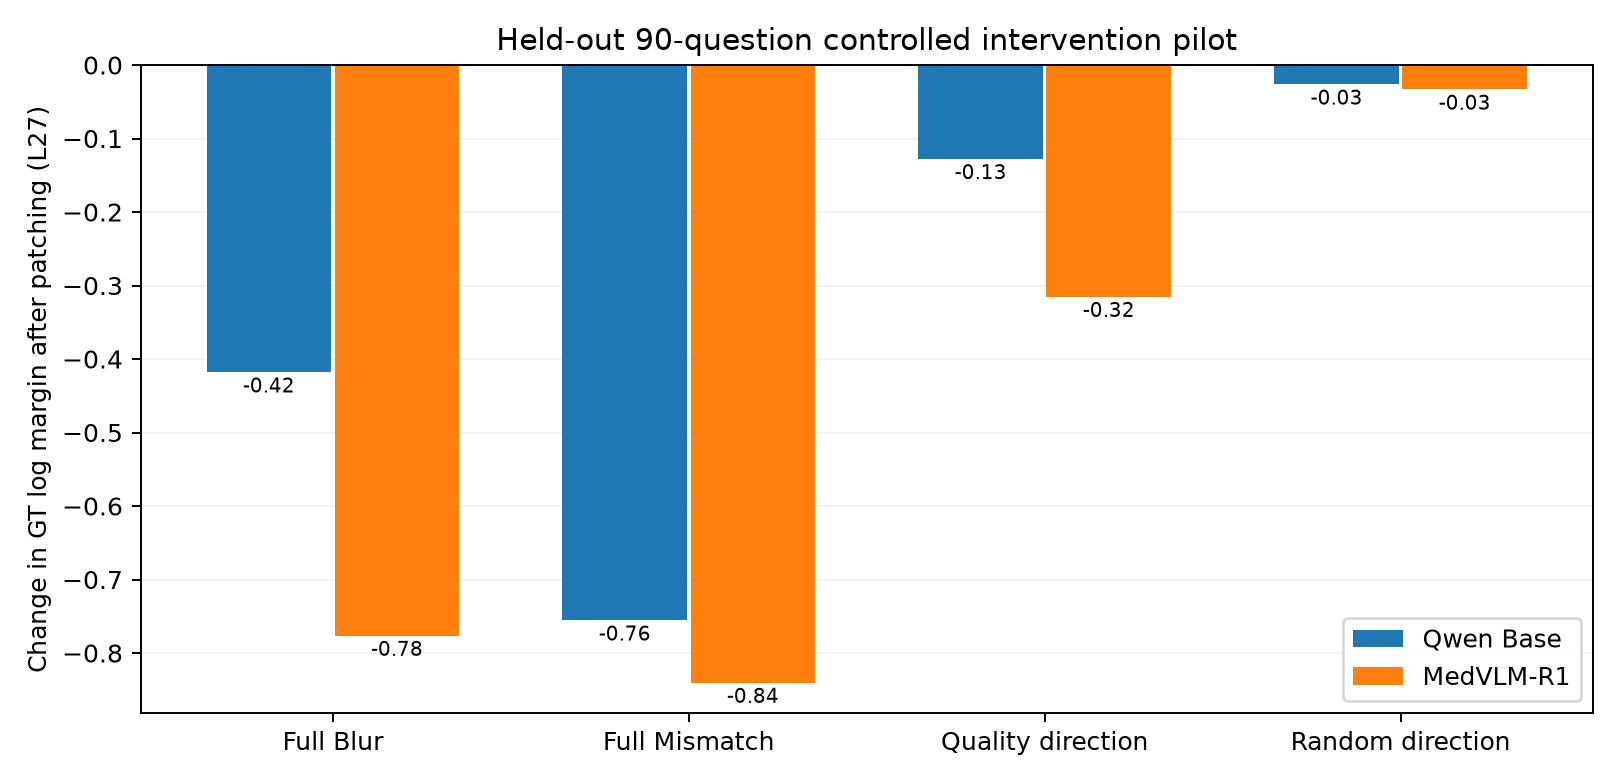
\includegraphics[keepaspectratio,alt={Effects of
full-state replacement and learned quality direction on Clean GT log
margin}]{figures/clean_log_margin_change.png}}
\caption{Effects of full-state replacement and learned quality direction
on Clean GT log margin}
\end{figure}

This experiment causally establishes that the intermediate
decision-state differences induced by Blur and Mismatch can alter
answers, including answers that were previously correct. Since the full
state carries both visual content and quality-related information, we
next test an aggregated \textbf{quality-associated direction}, learned
independently of the evaluation questions.

\subsubsection{2.8. Experiment C --- quality-associated direction and
visual-content
reliance}\label{experiment-c-quality-associated-direction-and-visual-content-reliance}

We selected a \textbf{stratified, disjoint split} from the official
dataset: \textbf{450 training questions} (150 per modality) to construct
candidate directions and \textbf{90 held-out evaluation questions} (30
per modality). The choice of samples is seeded and independent of model
correctness. Both checkpoints use the identical split and original O0
option order; all evaluations use matched image-processing settings. The
model weights remain fixed.

For each layer \(L\), we compute a candidate quality-change direction
from paired training-question representations:

\[d_{\mathrm{quality}}^{(L)}=\frac{1}{450}\sum_{i\in\mathrm{train}}\left(h_{i,\mathrm{Blur}}^{(L)}-h_{i,\mathrm{Clean}}^{(L)}\right).\]

We normalize this mean direction to \textbf{half the median
training-question Clean-to-Blur displacement norm}, then add it at the
decision-token residual position during inference:

\[h_{i,\mathrm{intervened}}^{(L)}=h_{i,\mathrm{input}}^{(L)}+\alpha\,\widetilde d_{\mathrm{quality}}^{(L)}.\]

The primary test uses \(\alpha=1\), corresponding to the frozen
half-median calibration. We also test \(\alpha=0.5\) and \(1.5\) as a
follow-up strength check. A random direction of identical norm serves as
a perturbation control. A separate Mismatch-associated direction is
derived by replacing Blur with the random same-modality Mismatch
condition in the training differences. The same learned quality
direction is injected while the actual visual input remains Clean,
Mismatch, or No-image, allowing effects on correct-image content to be
assessed directly.

The held-out per-sample Clean-to-Blur representation differences aligned
with the learned quality direction in \textbf{90.0\% (Base)} and
\textbf{94.4\% (RL)} of cases at L27, indicating a stable direction
across questions.

\textbf{Effect on Clean images (L27):}

{\def\LTcaptype{none} % do not increment counter
\begin{longtable}[]{@{}
  >{\raggedright\arraybackslash}p{(\linewidth - 6\tabcolsep) * \real{0.2000}}
  >{\raggedleft\arraybackslash}p{(\linewidth - 6\tabcolsep) * \real{0.2667}}
  >{\raggedleft\arraybackslash}p{(\linewidth - 6\tabcolsep) * \real{0.2667}}
  >{\raggedleft\arraybackslash}p{(\linewidth - 6\tabcolsep) * \real{0.2667}}@{}}
\toprule\noalign{}
\begin{minipage}[b]{\linewidth}\raggedright
Model
\end{minipage} & \begin{minipage}[b]{\linewidth}\raggedleft
Quality direction: Δ GT log margin
\end{minipage} & \begin{minipage}[b]{\linewidth}\raggedleft
Equal-norm random direction
\end{minipage} & \begin{minipage}[b]{\linewidth}\raggedleft
Quality direction: Δ answer entropy
\end{minipage} \\
\midrule\noalign{}
\endhead
\bottomrule\noalign{}
\endlastfoot
Qwen2-VL Base & \textbf{−0.128} & −0.026 & +0.071 \\
MedVLM-R1 & \textbf{−0.315} & −0.033 & +0.092 \\
\end{longtable}
}

The learned quality direction reduces the correct answer's margin and
increases uncertainty, with a larger effect than random perturbation.
The intervention at this strength changes few top-choice predictions:
\textbf{1/58} originally correct Base answers and \textbf{0/73}
originally correct RL answers flip after quality-direction injection at
L27. This distinguishes a \textbf{graded weakening of evidence} from the
larger decision disruption produced by full-state replacement.

\textbf{Does the quality direction reduce reliance on the \emph{correct
image content}?} For each held-out question, the learned direction is
applied separately to the Clean and the same-modality Mismatch forward
passes. We measure the change in their GT log-margin difference relative
to ordinary inference:

\[\Delta U_{\mathrm{content}}=\left[M_{\log}(\mathrm{Clean},\mathrm{patched})-M_{\log}(\mathrm{Mismatch},\mathrm{patched})\right]-\left[M_{\log}(\mathrm{Clean})-M_{\log}(\mathrm{Mismatch})\right].\]

{\def\LTcaptype{none} % do not increment counter
\begin{longtable}[]{@{}
  >{\raggedright\arraybackslash}p{(\linewidth - 4\tabcolsep) * \real{0.2727}}
  >{\raggedleft\arraybackslash}p{(\linewidth - 4\tabcolsep) * \real{0.3636}}
  >{\raggedleft\arraybackslash}p{(\linewidth - 4\tabcolsep) * \real{0.3636}}@{}}
\toprule\noalign{}
\begin{minipage}[b]{\linewidth}\raggedright
Intervention at L27
\end{minipage} & \begin{minipage}[b]{\linewidth}\raggedleft
Base: Δ content advantage (95\% CI)
\end{minipage} & \begin{minipage}[b]{\linewidth}\raggedleft
MedVLM-R1: Δ content advantage (95\% CI)
\end{minipage} \\
\midrule\noalign{}
\endhead
\bottomrule\noalign{}
\endlastfoot
\textbf{Learned quality direction} & \textbf{−0.131 {[}−0.193,
−0.071{]}} & \textbf{−0.157 {[}−0.231, −0.090{]}} \\
Equal-norm random direction & −0.028 {[}−0.049, −0.008{]} & −0.015
{[}−0.039, +0.008{]} \\
Quality minus random control & \textbf{−0.103 {[}−0.163, −0.049{]}} &
\textbf{−0.142 {[}−0.207, −0.082{]}} \\
Mismatch-associated direction & −0.022 {[}−0.058, +0.013{]} & −0.075
{[}−0.126, −0.026{]} \\
\end{longtable}
}

\begin{figure}
\centering
\pandocbounded{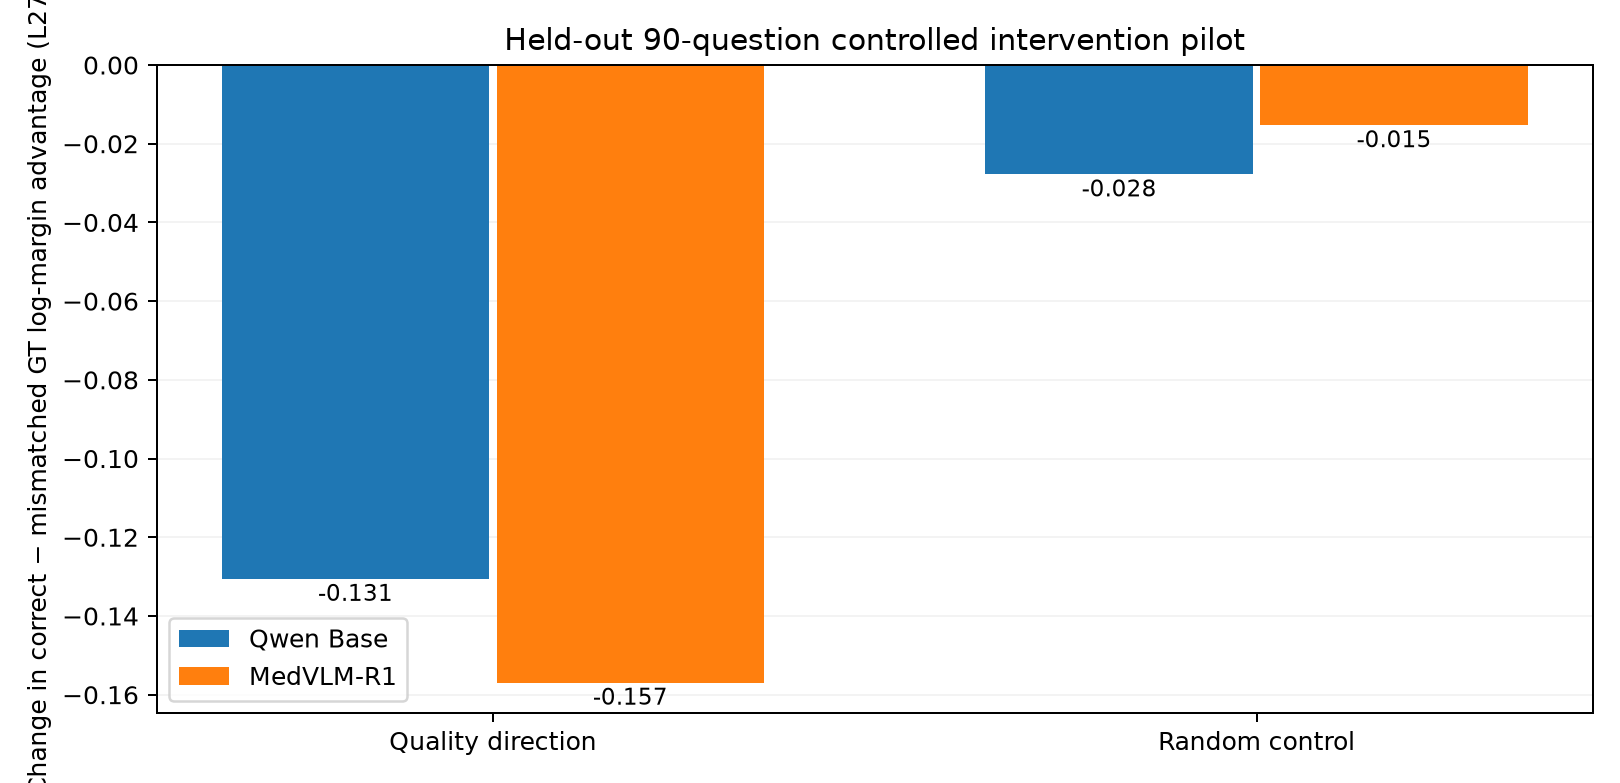
\includegraphics[keepaspectratio,alt={Quality-associated
versus random direction: change in correct-image
advantage}]{figures/visual_content_advantage_change.png}}
\caption{Quality-associated versus random direction: change in
correct-image advantage}
\end{figure}

A separate \textbf{No-image control} applies the same quality direction
when the question has no visual input. At L27, the GT log-margin change
is \textbf{+0.029 {[}−0.022, +0.079{]}} for Base and \textbf{−0.093
{[}−0.161, −0.025{]}} for RL. These shifts are smaller than the
corresponding changes on Clean images (\textbf{−0.128} and
\textbf{−0.315}), and the larger Clean-versus-Mismatch contrast
reduction is specific to the visual comparisons. The RL No-image effect
indicates that the learned direction can also influence non-visual
decision formation. Moreover, \textbf{No-image entropy rises by +0.095
in RL}, similar to its \textbf{+0.092 increase with Clean input} (Base:
+0.058 with No-image versus +0.071 with Clean). The learned direction
jointly alters \textbf{visual-content support and general answer
uncertainty}, motivating more selective causal probes.

We additionally examined the strength of the intervention at L27,
keeping the evaluation questions fixed:

{\def\LTcaptype{none} % do not increment counter
\begin{longtable}[]{@{}
  >{\raggedright\arraybackslash}p{(\linewidth - 4\tabcolsep) * \real{0.2727}}
  >{\raggedleft\arraybackslash}p{(\linewidth - 4\tabcolsep) * \real{0.3636}}
  >{\raggedleft\arraybackslash}p{(\linewidth - 4\tabcolsep) * \real{0.3636}}@{}}
\toprule\noalign{}
\begin{minipage}[b]{\linewidth}\raggedright
Quality-direction strength \(\alpha\)
\end{minipage} & \begin{minipage}[b]{\linewidth}\raggedleft
Base: Δ content advantage
\end{minipage} & \begin{minipage}[b]{\linewidth}\raggedleft
RL: Δ content advantage
\end{minipage} \\
\midrule\noalign{}
\endhead
\bottomrule\noalign{}
\endlastfoot
0.5 & −0.081 & −0.083 \\
1.0 & −0.131 & −0.157 \\
1.5 & −0.200 & −0.218 \\
\end{longtable}
}

\begin{figure}
\centering
\pandocbounded{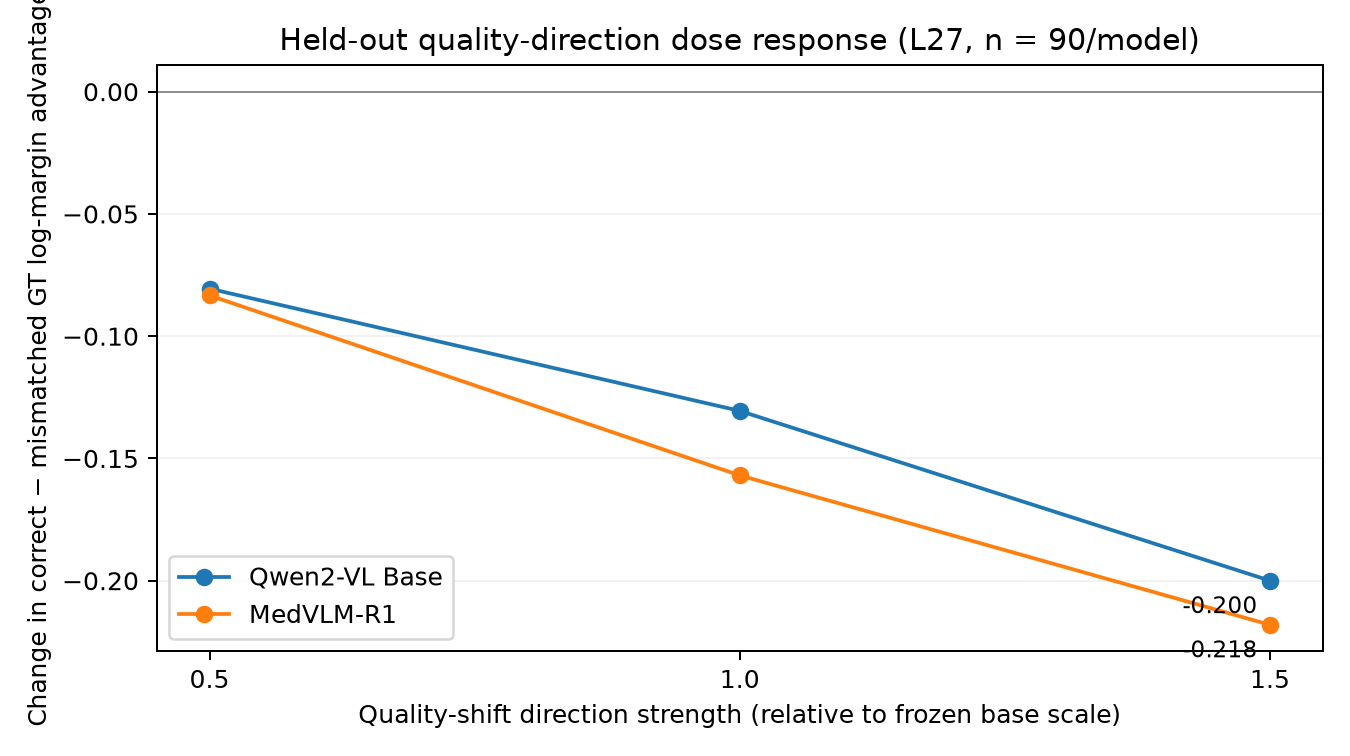
\includegraphics[keepaspectratio,alt={Quality-direction
strength and the resulting change in visual content
advantage}]{figures/quality_direction_dose_response.png}}
\caption{Quality-direction strength and the resulting change in visual
content advantage}
\end{figure}

The graded strength response, the held-out alignment of
quality-associated representation differences, and the smaller effects
of random directions provide converging evidence that this learned
direction \textbf{modulates the predictive contribution of visual
content}. The direction combines image-detail loss and
answer-uncertainty signals at the decision-token position. The next
mechanism experiment will isolate quality-sensitive subspaces while
controlling for image content and clinical diagnosability.

\subsubsection{2.9. Reproducibility and evaluation
scope}\label{reproducibility-and-evaluation-scope}

The new pilot uses released model checkpoints, the previously generated
matched-processing hidden representations and fixed donor assignments,
and the frozen O0 candidate-answer prompt. It updates \textbf{no model
weights} and transfers activations only \textbf{within each checkpoint}.
Direction construction is performed on 450 training questions; all 90
evaluation questions are held out. Identity/self-patch checks returned
\textbf{exactly zero GT log-margin change} at the tested layers in the
GPU runs.

All summary changes and intervals are derived from per-question
predictions. The primary run contains \textbf{2,610 scored intervention
records per checkpoint}. The No-image/Mismatch diagnostic adds
\textbf{630 records per checkpoint}, and the dose-response check adds
\textbf{360 records per checkpoint}. The experiment inputs and generated
outputs are kept in the
\href{https://github.com/bbuller591-sketch/medical-vlm-visual-reliance/tree/main/experiments/quality_state_interchange_20261009}{quality-intervention
analysis bundle}. The implementation includes
\href{https://github.com/bbuller591-sketch/medical-vlm-visual-reliance/blob/main/experiments/quality_state_interchange_20261009/scripts/run_interchange.py}{decision-token
interchange},
\href{https://github.com/bbuller591-sketch/medical-vlm-visual-reliance/blob/main/experiments/quality_state_interchange_20261009/scripts/analyze.py}{quality-direction
analysis}, and
\href{https://github.com/bbuller591-sketch/medical-vlm-visual-reliance/blob/main/experiments/quality_state_interchange_20261009/scripts/dose_response.py}{dose-response
analysis}. Numerical results, metadata, and plots are included. Full GPU
re-execution also uses the cached hidden-state arrays from the earlier
mechanism study, whose extraction scripts and model/data setup are
retained in the wider project.

\subsection{Appendix 3. Post-Training Gains and Non-Visual Medical VQA
Performance}\label{appendix-3.-post-training-gains-and-non-visual-medical-vqa-performance}

\subsubsection{3.1. Matched scoring: Clean versus
No-image}\label{matched-scoring-clean-versus-no-image}

The primary comparison uses the \textbf{825 questions that originally
have four answer choices}, including the full \textbf{300-question MRI}
set. The Base and RL checkpoints are evaluated with identical
candidate-score normalization, three answer-position arrangements
(original, cyclic shift, seeded permutation), the same semantic-answer
mapping, and the same item set. The accuracy numbers below average the
\textbf{correctness indicator across all three option orders} for every
question; each original question has equal weight.

The \textbf{image-presence benefit} is the within-checkpoint accuracy
difference between Clean and No-image:

\[B_{\mathrm{image}}(m)=\mathrm{Acc}_m(\mathrm{Clean})-\mathrm{Acc}_m(\mathrm{NoImage}).\]

The \textbf{RL gain} compares the two checkpoints under a fixed input
condition, and the change in image-presence benefit compares those two
gains:

\[\begin{aligned}
G(c)&=\mathrm{Acc}_{\mathrm{RL}}(c)-\mathrm{Acc}_{\mathrm{Base}}(c),\
\Delta B_{\mathrm{image}}&=B_{\mathrm{image}}(\mathrm{RL})-B_{\mathrm{image}}(\mathrm{Base})\
&=G(\mathrm{Clean})-G(\mathrm{NoImage}).
\end{aligned}\]

The accuracy values appear in the Part 3.1 compact table above. Below
are their \textbf{question-paired 95\% confidence intervals} and the
corresponding intervals for image-presence benefit:

{\def\LTcaptype{none} % do not increment counter
\begin{longtable}[]{@{}
  >{\raggedright\arraybackslash}p{(\linewidth - 6\tabcolsep) * \real{0.2000}}
  >{\raggedleft\arraybackslash}p{(\linewidth - 6\tabcolsep) * \real{0.2667}}
  >{\raggedleft\arraybackslash}p{(\linewidth - 6\tabcolsep) * \real{0.2667}}
  >{\raggedleft\arraybackslash}p{(\linewidth - 6\tabcolsep) * \real{0.2667}}@{}}
\toprule\noalign{}
\begin{minipage}[b]{\linewidth}\raggedright
Evaluation / model
\end{minipage} & \begin{minipage}[b]{\linewidth}\raggedleft
Clean accuracy: 95\% CI
\end{minipage} & \begin{minipage}[b]{\linewidth}\raggedleft
No-image accuracy: 95\% CI
\end{minipage} & \begin{minipage}[b]{\linewidth}\raggedleft
Image benefit: 95\% CI (pp)
\end{minipage} \\
\midrule\noalign{}
\endhead
\bottomrule\noalign{}
\endlastfoot
MRI 300 / Qwen Base & {[}62.89\%, 71.67\%{]} & {[}39.33\%, 47.89\%{]} &
{[}+18.78, +28.78{]} \\
MRI 300 / MedVLM-R1 & {[}94.67\%, 98.00\%{]} & {[}72.11\%, 79.22\%{]} &
{[}+17.22, +24.44{]} \\
All 825 / Qwen Base & {[}66.22\%, 71.64\%{]} & {[}41.54\%, 46.67\%{]} &
{[}+21.74, +27.80{]} \\
All 825 / MedVLM-R1 & {[}78.59\%, 83.31\%{]} & {[}55.35\%, 60.48\%{]} &
{[}+20.28, +25.78{]} \\
\end{longtable}
}

{\def\LTcaptype{none} % do not increment counter
\begin{longtable}[]{@{}
  >{\raggedright\arraybackslash}p{(\linewidth - 6\tabcolsep) * \real{0.2000}}
  >{\raggedleft\arraybackslash}p{(\linewidth - 6\tabcolsep) * \real{0.2667}}
  >{\raggedleft\arraybackslash}p{(\linewidth - 6\tabcolsep) * \real{0.2667}}
  >{\raggedleft\arraybackslash}p{(\linewidth - 6\tabcolsep) * \real{0.2667}}@{}}
\toprule\noalign{}
\begin{minipage}[b]{\linewidth}\raggedright
Evaluation set
\end{minipage} & \begin{minipage}[b]{\linewidth}\raggedleft
RL Clean gain: 95\% CI (pp)
\end{minipage} & \begin{minipage}[b]{\linewidth}\raggedleft
RL No-image gain: 95\% CI (pp)
\end{minipage} & \begin{minipage}[b]{\linewidth}\raggedleft
Change in image benefit (95\% CI, pp)
\end{minipage} \\
\midrule\noalign{}
\endhead
\bottomrule\noalign{}
\endlastfoot
MRI 300 & {[}+24.89, +33.44{]} & {[}+28.00, +36.33{]} & \textbf{−3.00}
{[}−7.56, +1.67{]} \\
All 825 & {[}+10.06, +14.14{]} & {[}+11.84, +15.84{]} & \textbf{−1.74}
{[}−3.80, +0.32{]} \\
\end{longtable}
}

\begin{figure}
\centering
\pandocbounded{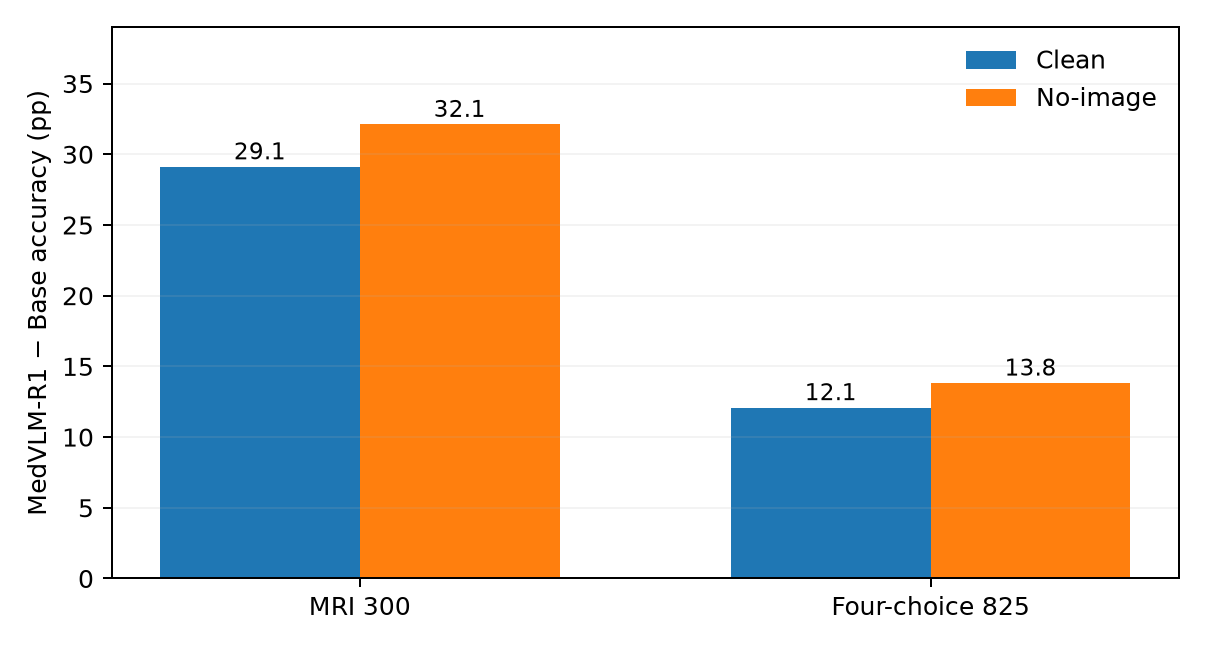
\includegraphics[keepaspectratio,alt={Post-training
improvement with and without the image}]{figures/post_rl_uplift.png}}
\caption{Post-training improvement with and without the image}
\end{figure}

The intervals are \textbf{10,000 question-paired bootstrap resamples}
(seed 20261009), preserving each question's three option-order
observations as a single resampling unit. On MRI, the Base-to-RL Clean
improvement was 29.11 pp, while its No-image improvement was 32.11
pp.~The corresponding values for the full four-choice evaluation were
12.08 pp and 13.82 pp.~The small negative differences in image-presence
benefit have intervals spanning zero; the central finding is the
\textbf{large improvement under No-image input}.

\textbf{Non-visual benchmarks.} With no image, Base achieved
\textbf{44.12\%} on the 825 four-choice questions, versus \textbf{25\%}
uniform random selection. The original answer-position distribution for
these items is A=217, B=191, C=213, D=204; always choosing the most
common answer letter yields \textbf{26.30\%}. Thus, the No-image
baseline exploits information beyond a fixed answer-position preference.
The measured non-visual signal combines medical domain knowledge, option
wording, and dataset-specific question patterns.

\subsubsection{3.2. Where are the gains concentrated? MRI versus CT and
X-ray}\label{where-are-the-gains-concentrated-mri-versus-ct-and-x-ray}

The
\href{https://papers.miccai.org/miccai-2025/paper/3267_paper.pdf}{MedVLM-R1
paper} describes GRPO post-training on \textbf{600 MRI training
examples}, evaluating \textbf{300 MRI} questions in-domain and
\textbf{300 CT plus 300 X-ray} questions as out-of-training-modality
tests. The matched four-choice subset retains 237 CT questions and 288
X-ray questions. Breaking down the matched candidate-scoring results
shows where the gains occur:

{\def\LTcaptype{none} % do not increment counter
\begin{longtable}[]{@{}
  >{\raggedright\arraybackslash}p{(\linewidth - 8\tabcolsep) * \real{0.1579}}
  >{\raggedleft\arraybackslash}p{(\linewidth - 8\tabcolsep) * \real{0.2105}}
  >{\raggedleft\arraybackslash}p{(\linewidth - 8\tabcolsep) * \real{0.2105}}
  >{\raggedleft\arraybackslash}p{(\linewidth - 8\tabcolsep) * \real{0.2105}}
  >{\raggedleft\arraybackslash}p{(\linewidth - 8\tabcolsep) * \real{0.2105}}@{}}
\toprule\noalign{}
\begin{minipage}[b]{\linewidth}\raggedright
Modality (four-choice only)
\end{minipage} & \begin{minipage}[b]{\linewidth}\raggedleft
RL gain: Clean
\end{minipage} & \begin{minipage}[b]{\linewidth}\raggedleft
RL gain: No-image
\end{minipage} & \begin{minipage}[b]{\linewidth}\raggedleft
Base image benefit
\end{minipage} & \begin{minipage}[b]{\linewidth}\raggedleft
RL image benefit
\end{minipage} \\
\midrule\noalign{}
\endhead
\bottomrule\noalign{}
\endlastfoot
\textbf{MRI (n=300)} & \textbf{+29.11 pp} & \textbf{+32.11 pp} & +23.78
pp & +20.78 pp \\
CT (n=237) & +4.36 pp & +5.49 pp & +19.69 pp & +18.57 pp \\
X-ray (n=288) & +0.69 pp & +1.62 pp & +29.98 pp & +29.05 pp \\
\end{longtable}
}

Both the Clean and the No-image improvements are strongest on
\textbf{MRI}, the training modality. The image-presence benefit is
substantial for all three modalities, and the additional RL gain is
disproportionately concentrated on MRI. This makes \textbf{MRI-specific
non-visual knowledge and question--option patterns} important candidate
explanations to examine in subsequent experiments.

\subsubsection{3.3. Matched 559-item joint-Clean-correct
subset}\label{matched-559-item-joint-clean-correct-subset}

\textbf{Selection and protocol.} We used the \textbf{559 fixed
questions} chosen from the 825 four-option items for which Qwen Base and
MedVLM-R1 both predict the original ground truth correctly with the
original Clean image. These 559 questions are \textbf{MRI 207, CT 160,
and X-ray 192}. Crucially, the cohort uses \textbf{matched normalized
candidate scoring with the original option order (O0)} for \emph{both}
models. This differs from the older 506-item native-generated versus
direct-scored diagnostic. We reuse the \textbf{no-hint Clean and
No-image} evaluations of the complete 559-item advice dataset; no hinted
responses enter this analysis. The item IDs were frozen by Clean
correctness before checking No-image behavior. Both models are evaluated
on exactly the same items.

{\def\LTcaptype{none} % do not increment counter
\begin{longtable}[]{@{}
  >{\raggedright\arraybackslash}p{(\linewidth - 6\tabcolsep) * \real{0.2000}}
  >{\raggedleft\arraybackslash}p{(\linewidth - 6\tabcolsep) * \real{0.2667}}
  >{\raggedleft\arraybackslash}p{(\linewidth - 6\tabcolsep) * \real{0.2667}}
  >{\raggedleft\arraybackslash}p{(\linewidth - 6\tabcolsep) * \real{0.2667}}@{}}
\toprule\noalign{}
\begin{minipage}[b]{\linewidth}\raggedright
Subset
\end{minipage} & \begin{minipage}[b]{\linewidth}\raggedleft
Qwen Base No-image
\end{minipage} & \begin{minipage}[b]{\linewidth}\raggedleft
R1 No-image
\end{minipage} & \begin{minipage}[b]{\linewidth}\raggedleft
R1 − Base (95\% paired CI, pp)
\end{minipage} \\
\midrule\noalign{}
\endhead
\bottomrule\noalign{}
\endlastfoot
\textbf{All 559} & 288/559 (51.52\%) & \textbf{348/559 (62.25\%)} &
\textbf{+10.73} {[}+7.87, +13.60{]} \\
MRI 207 & 95/207 (45.89\%) & \textbf{148/207 (71.50\%)} &
\textbf{+25.60} {[}+19.81, +31.40{]} \\
CT 160 & 98/160 (61.25\%) & 104/160 (65.00\%) & +3.75 {[}0.00,
+7.50{]} \\
X-ray 192 & 95/192 (49.48\%) & 96/192 (50.00\%) & +0.52 {[}−2.60,
+3.65{]} \\
\end{longtable}
}

\textbf{Paired No-image outcomes, all 559:} both correct \textbf{282},
only R1 correct \textbf{66}, only Base correct \textbf{6}, both
incorrect \textbf{205}. Intervals above use \textbf{10,000
question-paired bootstrap resamples (seed 20261010)}. The same original
answer choices and gold labels are evaluated under image removal. The
computed totals and per-modality CIs are frozen in
\href{https://github.com/bbuller591-sketch/medical-vlm-visual-reliance/blob/main/results/joint_clean_559_noimage_audit.json}{\texttt{joint\_clean\_559\_noimage\_audit.json}},
regenerated without GPU from
\href{https://github.com/bbuller591-sketch/medical-vlm-visual-reliance/blob/main/scripts/analyze_joint_clean_559.py}{\texttt{analyze\_joint\_clean\_559.py}}
and the completed
\href{https://github.com/bbuller591-sketch/medical-vlm-visual-reliance/blob/main/experiments/visual_advice_conflict_20261009/README.md}{\texttt{559-item\ advice\ experiment}}.

\textbf{Interpretation.} R1's No-image advantage persists on questions
\textbf{already answered correctly by both models with the original
image}, extending the gain to previously shared Clean successes. The
effect is concentrated in MRI and aligns with an accuracy reward that
reinforces answer-predictive medical knowledge, option associations, and
benchmark regularities. \textbf{Reward-amplified use of these non-visual
patterns is the leading explanation for the retained accuracy
advantage.} The all-825 analysis in Appendix 3.1 independently shows
similarly large RL gains with and without images.

\subsubsection{3.4. Questions both checkpoints already answered
correctly with Clean
images}\label{questions-both-checkpoints-already-answered-correctly-with-clean-images}

As a \textbf{historical supplementary check}, we revisit the \textbf{506
four-choice questions on which both checkpoints were correct with their
original Clean images} (192 MRI, 137 CT, 177 X-ray). They were selected
using only Clean correctness, before examining No-image or image
perturbations. This creates a focused diagnostic: among questions both
checkpoints can solve when supplied the intended image, \textbf{which
answers can still be recovered without the image?}

Among the \textbf{499 questions with a valid No-image response from both
models}, we observed:

{\def\LTcaptype{none} % do not increment counter
\begin{longtable}[]{@{}lrr@{}}
\toprule\noalign{}
No-image outcome on the same 499 questions & Count & Share of 499 \\
\midrule\noalign{}
\endhead
\bottomrule\noalign{}
\endlastfoot
Both correct & 219 & 43.9\% \\
\textbf{RL correct, Base incorrect} & \textbf{82} & \textbf{16.4\%} \\
Base correct, RL incorrect & 46 & 9.2\% \\
Both incorrect & 152 & 30.5\% \\
\end{longtable}
}

Consequently, RL retained \textbf{301/499 (60.32\%)} No-image correct
answers, while Base retained \textbf{265/499 (53.11\%)}, a paired
difference of \textbf{+7.21 pp} (95\% bootstrap CI \textbf{{[}+2.81,
+11.62{]} pp}). In this original 506-item diagnostic, the MedVLM-R1
Clean selection and No-image outcomes used \textbf{native generated
answers}, whereas the Base used \textbf{direct candidate scoring}. We
use this subset to understand \emph{answer retention after image
removal}; the matched full-set experiment in Appendix 3.1 and the new
matched joint-Clean-correct analysis in Appendix 3.3 provide the primary
like-for-like checkpoint comparisons.

This older 506-item diagnostic is informative because correct Clean
performance is shared by the two models. This allows a direct comparison
of how often each checkpoint can reproduce a previously successful
answer without the image. Image-based success can come from recognizing
the image, existing medical knowledge, or both; the No-image comparison
reveals how strongly successful answers persist when current visual
content is removed.

A further breakdown from the original 825-item experiment supports the
same task-conditional interpretation:

{\def\LTcaptype{none} % do not increment counter
\begin{longtable}[]{@{}
  >{\raggedright\arraybackslash}p{(\linewidth - 6\tabcolsep) * \real{0.2000}}
  >{\raggedleft\arraybackslash}p{(\linewidth - 6\tabcolsep) * \real{0.2667}}
  >{\raggedleft\arraybackslash}p{(\linewidth - 6\tabcolsep) * \real{0.2667}}
  >{\raggedleft\arraybackslash}p{(\linewidth - 6\tabcolsep) * \real{0.2667}}@{}}
\toprule\noalign{}
\begin{minipage}[b]{\linewidth}\raggedright
Clean-correctness group
\end{minipage} & \begin{minipage}[b]{\linewidth}\raggedleft
Number of questions
\end{minipage} & \begin{minipage}[b]{\linewidth}\raggedleft
RL No-image accuracy
\end{minipage} & \begin{minipage}[b]{\linewidth}\raggedleft
Base No-image accuracy
\end{minipage} \\
\midrule\noalign{}
\endhead
\bottomrule\noalign{}
\endlastfoot
Both Clean-correct & 506 & 60.3\% & 53.2\% \\
RL-only Clean-correct & 162 & 71.4\% & 25.3\% \\
Base-only Clean-correct & 25 & 24.0\% & 48.0\% \\
Neither Clean-correct & 127 & 25.2\% & 26.8\% \\
\end{longtable}
}

The 506-question conditional groups measure \textbf{how often each
checkpoint preserves already-correct answers after image removal}. The
convergence of its pattern with Appendix 3.1 motivates the
training-reward analysis below.

\subsubsection{3.5. Why the MedVLM-R1 reward motivates a non-visual
prior
hypothesis}\label{why-the-medvlm-r1-reward-motivates-a-non-visual-prior-hypothesis}

According to
\href{https://papers.miccai.org/miccai-2025/paper/3267_paper.pdf}{MedVLM-R1
(MICCAI 2025), Section 3}, its \textbf{Group Relative Policy
Optimization (GRPO)} training uses two rule-based reward components for
medical multiple-choice VQA:

{\def\LTcaptype{none} % do not increment counter
\begin{longtable}[]{@{}
  >{\raggedright\arraybackslash}p{(\linewidth - 2\tabcolsep) * \real{0.5000}}
  >{\raggedright\arraybackslash}p{(\linewidth - 2\tabcolsep) * \real{0.5000}}@{}}
\toprule\noalign{}
\begin{minipage}[b]{\linewidth}\raggedright
Reward component
\end{minipage} & \begin{minipage}[b]{\linewidth}\raggedright
What is rewarded
\end{minipage} \\
\midrule\noalign{}
\endhead
\bottomrule\noalign{}
\endlastfoot
\textbf{Format reward} & The required structured reasoning/final-answer
tags and response format \\
\textbf{Accuracy reward} & Agreement of the final chosen answer with the
reference option, with full or partial credit according to answer
format \\
\end{longtable}
}

The overall reward is the sum of the two components, each up to one
point. The format component encourages a structured explanation and
answer; the accuracy component rewards choosing the target option.
\textbf{Neither component directly evaluates whether the output causally
depends on the current medical image or cites correct image-specific
evidence.}

\textbf{The reward creates a direct incentive to fit whichever patterns
predict the correct option.} In medical MCQs, those patterns include
genuine image findings but also medical knowledge, answer-option
plausibility, recurring question structures, and dataset-specific label
associations. The experiments show where the reward-aligned, non-visual
route becomes especially effective: MRI No-image accuracy rises from
\textbf{43.56\% to 75.67\%}, and the MRI-focused advantage remains
\textbf{+25.60 pp} within the jointly Clean-correct 559-item cohort.
\textbf{Reward-driven exploitation of these non-visual regularities is
therefore a central explanation of the post-training gains.}

The distinction is visible across three measurements: \textbf{Clean RL
gain} (+12.08 pp overall), \textbf{No-image RL gain} (+13.82 pp
overall), and \textbf{change in the image-presence benefit} (−1.74 pp,
paired 95\% CI {[}−3.80, +0.32{]}). \textbf{The reward improves answer
prediction substantially even in the absence of current visual
evidence.} A reward specifically targeting visual-evidence reliability
would instead evaluate whether the model changes its answer
appropriately when the image's diagnostic information or quality
changes.

\subsubsection{3.6. Follow-up experiment: image-free RL under a matched
training
design}\label{follow-up-experiment-image-free-rl-under-a-matched-training-design}

To test the learning mechanism more directly, a controlled experiment
could start with the \textbf{same Qwen2-VL Base checkpoint} and matched
MRI training examples, then compare: (a) the original image-conditioned
RL training protocol and (b) the \textbf{same RL objective with medical
images omitted during training}. Both branches would match the
optimizer, reward, training question/answer labels, and step budget.
Evaluation would include Clean, No-image, Mismatch, and degraded-image
variants on held-out questions, plus external medical benchmarks.

This design directly tests how much of the RL gain can be reproduced
through text-only training and whether image-conditioned RL delivers
additional sensitivity to correct visual content. This planned
training-level control complements the completed released-checkpoint
evaluations in Appendix 3.1--3.5.

\textbf{Reproducibility.} The
\href{https://github.com/bbuller591-sketch/medical-vlm-visual-reliance/blob/main/results/official825_scores.csv}{matched
per-order accuracy records} and
\href{https://github.com/bbuller591-sketch/medical-vlm-visual-reliance/blob/main/results/rl_matched_gains_audit.json}{item-paired
bootstrap audit} support Appendix 3.1--3.2, regenerated by
\href{https://github.com/bbuller591-sketch/medical-vlm-visual-reliance/blob/main/scripts/analyze_rl_gains.py}{\texttt{analyze\_rl\_gains.py}}.
The 506-question group counts come from the original analysis records in
the project, with released aggregate retention results in
\href{https://github.com/bbuller591-sketch/medical-vlm-visual-reliance/blob/main/results/clean_correct_506_interventions.csv}{\texttt{clean\_correct\_506\_interventions.csv}}.
All percentages are reported in \textbf{percentage points (pp)} when
subtracting accuracies.

\subsection{Appendix 4. External Generalization and Evidence-Conflict
Evaluation}\label{appendix-4.-external-generalization-and-evidence-conflict-evaluation}

\subsubsection{4.1. External datasets and matched
evaluation}\label{external-datasets-and-matched-evaluation}

The main external comparison holds both released checkpoints fixed:
\textbf{Qwen2-VL-2B-Instruct} (Base) and \textbf{MedVLM-R1} (RL).
\textbf{SLAKE English Yes/No test} contains 355 questions over
\textbf{96 unique images}, with two candidate answers. \textbf{PMC-VQA}
uses a frozen, label-stratified sample of 1,000 four-option questions
over \textbf{852 unique images} from its curated test split. Every item
uses \textbf{Clean}, \textbf{No-image} (no image tokens), and
\textbf{Shuffled-image} (a frozen, seeded different-item donor image).
Question text, options, and original reference labels remain fixed. Both
models are evaluated on identical questions and assigned donors.
Candidate-option probabilities are normalized and mapped to semantic
answers across \textbf{two option orders for SLAKE} and \textbf{three
orders for PMC-VQA}.

The \textbf{Clean − No-image} contrast tracks the value of supplying an
image-containing input; \textbf{Clean − Shuffled} tracks the value of
the \emph{correct image content} while retaining a real image in both
conditions. Paired confidence intervals resample \textbf{source images
as clusters}, since several questions share a source image. Each
question contributes its option-order-averaged accuracy. The official
825-question and MRI results in Parts 3--4 use their separate matched
three-order evaluation and are compared as \textbf{within-dataset
checkpoint gains}.

\subsubsection{4.2. External accuracy, effect sizes, and confidence
intervals}\label{external-accuracy-effect-sizes-and-confidence-intervals}

{\def\LTcaptype{none} % do not increment counter
\begin{longtable}[]{@{}
  >{\raggedright\arraybackslash}p{(\linewidth - 10\tabcolsep) * \real{0.1304}}
  >{\raggedleft\arraybackslash}p{(\linewidth - 10\tabcolsep) * \real{0.1739}}
  >{\raggedleft\arraybackslash}p{(\linewidth - 10\tabcolsep) * \real{0.1739}}
  >{\raggedleft\arraybackslash}p{(\linewidth - 10\tabcolsep) * \real{0.1739}}
  >{\raggedleft\arraybackslash}p{(\linewidth - 10\tabcolsep) * \real{0.1739}}
  >{\raggedleft\arraybackslash}p{(\linewidth - 10\tabcolsep) * \real{0.1739}}@{}}
\toprule\noalign{}
\begin{minipage}[b]{\linewidth}\raggedright
Dataset / checkpoint
\end{minipage} & \begin{minipage}[b]{\linewidth}\raggedleft
Clean accuracy
\end{minipage} & \begin{minipage}[b]{\linewidth}\raggedleft
No-image accuracy
\end{minipage} & \begin{minipage}[b]{\linewidth}\raggedleft
Shuffled accuracy
\end{minipage} & \begin{minipage}[b]{\linewidth}\raggedleft
Clean − No-image
\end{minipage} & \begin{minipage}[b]{\linewidth}\raggedleft
Clean − Shuffled
\end{minipage} \\
\midrule\noalign{}
\endhead
\bottomrule\noalign{}
\endlastfoot
SLAKE / Base & 68.03\% & 45.35\% & 52.82\% & +22.68 pp & +15.21 pp \\
SLAKE / R1 & 62.25\% & 42.68\% & 49.15\% & +19.58 pp & +13.10 pp \\
PMC-VQA / Base & 45.10\% & 31.43\% & 29.33\% & +13.67 pp & +15.77 pp \\
PMC-VQA / R1 & 45.43\% & 31.07\% & 29.40\% & +14.37 pp & +16.03 pp \\
\end{longtable}
}

{\def\LTcaptype{none} % do not increment counter
\begin{longtable}[]{@{}
  >{\raggedright\arraybackslash}p{(\linewidth - 6\tabcolsep) * \real{0.2000}}
  >{\raggedleft\arraybackslash}p{(\linewidth - 6\tabcolsep) * \real{0.2667}}
  >{\raggedleft\arraybackslash}p{(\linewidth - 6\tabcolsep) * \real{0.2667}}
  >{\raggedleft\arraybackslash}p{(\linewidth - 6\tabcolsep) * \real{0.2667}}@{}}
\toprule\noalign{}
\begin{minipage}[b]{\linewidth}\raggedright
Dataset
\end{minipage} & \begin{minipage}[b]{\linewidth}\raggedleft
RL − Base Clean (95\% CI, pp)
\end{minipage} & \begin{minipage}[b]{\linewidth}\raggedleft
RL − Base No-image (95\% CI, pp)
\end{minipage} & \begin{minipage}[b]{\linewidth}\raggedleft
Change in correct-image benefit: (RL − Base) in Clean − Shuffled (95\%
CI, pp)
\end{minipage} \\
\midrule\noalign{}
\endhead
\bottomrule\noalign{}
\endlastfoot
\textbf{SLAKE} & \textbf{−5.77} {[}−9.09, −2.51{]} & \textbf{−2.68}
{[}−4.40, −1.04{]} & −2.11 {[}−5.10, +0.68{]} \\
\textbf{PMC-VQA} & +0.33 {[}−0.57, +1.24{]} & −0.37 {[}−1.24, +0.53{]} &
+0.27 {[}−0.90, +1.41{]} \\
\end{longtable}
}

The reference answer frequencies are \textbf{180 Yes / 175 No} on SLAKE
(50.70\% majority baseline) and \textbf{31.9\% majority-choice prior} on
the stratified PMC-VQA set (uniform four-way chance: 25\%). R1's
original MRI gains of \textbf{+29.11 pp Clean} and \textbf{+32.11 pp
No-image} contrast with the sharply smaller external gains. The complete
aggregate audit, including source-image clustered bootstrap intervals,
is in
\href{https://github.com/bbuller591-sketch/medical-vlm-visual-reliance/blob/main/results/external_base_rl_generalization_audit.json}{\texttt{external\_base\_rl\_generalization\_audit.json}}.

\subsubsection{4.3. Jointly Clean-correct questions on external
data}\label{jointly-clean-correct-questions-on-external-data}

As in Part 3.3, selection is performed from \textbf{Clean correct
predictions by both models}, followed by analysis of No-image
predictions for the \textbf{same questions}. Each dataset keeps its own
fixed candidate-scoring and option-order protocol.

{\def\LTcaptype{none} % do not increment counter
\begin{longtable}[]{@{}
  >{\raggedright\arraybackslash}p{(\linewidth - 6\tabcolsep) * \real{0.2000}}
  >{\raggedleft\arraybackslash}p{(\linewidth - 6\tabcolsep) * \real{0.2667}}
  >{\raggedleft\arraybackslash}p{(\linewidth - 6\tabcolsep) * \real{0.2667}}
  >{\raggedleft\arraybackslash}p{(\linewidth - 6\tabcolsep) * \real{0.2667}}@{}}
\toprule\noalign{}
\begin{minipage}[b]{\linewidth}\raggedright
Dataset / jointly Clean-correct set
\end{minipage} & \begin{minipage}[b]{\linewidth}\raggedleft
Base No-image correct
\end{minipage} & \begin{minipage}[b]{\linewidth}\raggedleft
MedVLM-R1 No-image correct
\end{minipage} & \begin{minipage}[b]{\linewidth}\raggedleft
RL − Base
\end{minipage} \\
\midrule\noalign{}
\endhead
\bottomrule\noalign{}
\endlastfoot
Original MRI / 207 & 95/207 (45.89\%) & \textbf{148/207 (71.50\%)} &
\textbf{+25.60 pp} \\
SLAKE / 209 & 91/209 (43.54\%) & 89/209 (42.58\%) & −0.96 pp \\
PMC-VQA / 448 & 252/448 (56.25\%) & 249/448 (55.58\%) & −0.67 pp \\
\end{longtable}
}

The original MRI advantage is large and persistent in the jointly
solvable subset; the SLAKE and PMC-VQA comparisons are nearly tied. This
pattern directly demonstrates \textbf{training-benchmark concentration
in R1's enhanced non-visual answer recovery}.

\subsubsection{4.4. Image-content relevance and opposite-label
pairs}\label{image-content-relevance-and-opposite-label-pairs}

The \textbf{Clean − Shuffled} content advantages in Appendix 4.2 show
substantial benefits from matching the image to the question on both
SLAKE and PMC-VQA. For SLAKE, an additional evidence-conflict audit
matched images with \textbf{identical normalized question text, matching
modality, and opposite reference Yes/No labels}, excluding
dataset-tagged knowledge-only items. We retained \textbf{47
distinct-image pairs} covering \textbf{21 question-by-modality groups}.
This holds the linguistic question fixed and uses the dataset's
annotated image-specific answer variation.

{\def\LTcaptype{none} % do not increment counter
\begin{longtable}[]{@{}
  >{\raggedright\arraybackslash}p{(\linewidth - 4\tabcolsep) * \real{0.2727}}
  >{\raggedleft\arraybackslash}p{(\linewidth - 4\tabcolsep) * \real{0.3636}}
  >{\raggedleft\arraybackslash}p{(\linewidth - 4\tabcolsep) * \real{0.3636}}@{}}
\toprule\noalign{}
\begin{minipage}[b]{\linewidth}\raggedright
Same-question, opposite-label SLAKE pairs
\end{minipage} & \begin{minipage}[b]{\linewidth}\raggedleft
Qwen Base
\end{minipage} & \begin{minipage}[b]{\linewidth}\raggedleft
MedVLM-R1
\end{minipage} \\
\midrule\noalign{}
\endhead
\bottomrule\noalign{}
\endlastfoot
Directionally correct shift in \(P(\mathrm{Yes})\) & 40/47
(\textbf{85.11\%}) & 38/47 (\textbf{80.85\%}) \\
Both image-specific answers correct & 24/47 (51.06\%) & 23/47
(48.94\%) \\
Mean \(P(\mathrm{Yes})\) shift (Yes-image minus No-image) & +0.314 &
+0.321 \\
\end{longtable}
}

The paired-image intervention directly measures the model's response to
a \textbf{label-changing image swap under fixed wording}. Both models
respond to the image content; R1 shows \textbf{no increase in
directional consistency or jointly correct responses}. Pair labels come
from SLAKE's dataset annotations. Individual examples and the paired
matching records are available in the source external-evaluation
analysis; the aggregate data appear in
\href{https://github.com/bbuller591-sketch/medical-vlm-visual-reliance/blob/main/results/external_base_rl_generalization_audit.json}{\texttt{external\_base\_rl\_generalization\_audit.json}}.

\subsubsection{4.5. Supplementary VQA-RAD transfer and cross-dataset
interpretation}\label{supplementary-vqa-rad-transfer-and-cross-dataset-interpretation}

The earlier \textbf{VQA-RAD closed Yes/No} test comprises \textbf{251
questions over 135 images}. Under its earlier, separately standardized
candidate-scoring setup, Base reaches \textbf{61.75\% Clean / 51.79\%
No-image / 58.96\% Shuffled}, and R1 reaches \textbf{63.55\% / 54.78\% /
58.57\%}. The resulting RL−Base differences are \textbf{+1.80 pp Clean}
and \textbf{+2.99 pp No-image}. Correct-image content benefit is
\textbf{+2.79 pp} for Base and \textbf{+4.98 pp} for R1; the
source-image clustered 95\% intervals for these content advantages are
{[}−3.81, +9.17{]} pp and {[}−0.38, +10.20{]} pp, respectively.

These modest VQA-RAD differences follow the same overarching external
pattern: the substantial original MRI gain \textbf{is absent from this
additional test set}. VQA-RAD uses a distinct existing scoring setup and
is reported separately from the matched SLAKE/PMC-VQA evaluation.
SLAKE's paired images and PMC-VQA's shuffled-image comparison
additionally show how benchmark content and repeated question formats
determine the diagnostic strength of a visual intervention.

\textbf{Sources and reproduction.} The portable external aggregate
summary is
\href{https://github.com/bbuller591-sketch/medical-vlm-visual-reliance/blob/main/results/external_base_rl_generalization_audit.json}{external
generalization data}. The
\href{https://github.com/bbuller591-sketch/medical-vlm-visual-reliance/blob/main/scripts/evaluate_external.py}{external
model evaluator} and
\href{https://github.com/bbuller591-sketch/medical-vlm-visual-reliance/blob/main/scripts/analyze_inference.py}{paired
analysis implementation} provide the released evaluation pipeline. The
fixed SLAKE and PMC-VQA experiment outputs, opposite-label pair audit,
and VQA-RAD results remain in the project's external-evaluation archive.
This appendix uses the original fixed full evaluation sets and their
paired image controls.

\end{document}
